
\section{Results and Analysis}
\label{sec:Study Results}

We now present the results of our study and answer our five research questions. 

\subsection{\textbf{RQ1:} \textit{\RQOne}}

\paragraph{\textbf{Motivation}} Understanding the evolution of patterns is important because it can help developers to identify and circumvent risky design patterns and prevent the appearance of design anti-patterns \cite{jaafar2014anti}. While some tools can find software entities and their evolution patterns automatically, \eg{} \cite{van2002java,lanza2007object,rapu2004using,vaucher2009tracking}, no previous work investigated the mutation of design (anti-)patterns.

\paragraph{\textbf{Computing probability values for all possible mutations}} We apply the detection tools described in Section \ref{sec:Methodology} on snapshots of each of the systems listed in Table \ref{tab:StudySystems}. Each snapshot contains a large number of classes, which may participate in different types of design anti-patterns and--or design patterns. 

We take snapshots every 500 commits in the evolution histories of the systems. This commit interval period is adequate to detect changes occurring between two subsequent snapshots \cite{hassan2009predicting,canfora2010exploratory}.

We automatically compare each two subsequent snapshots to compute the numbers of added or deleted occurrences of design patterns and design anti-patterns. We build one Markov model for each system to show the probabilities of mutations between design patterns and design anti-patterns.

\begin{landscape}
\begin{table*}
\caption{Change probabilities of design anti-patterns and design patterns in Eclipse IDE}
\setlength\tabcolsep{0.08cm}
\scriptsize
\centering
\scalebox{0.73}{
{\renewcommand{\arraystretch}{1.05}
\begin{tabular}
{|l|l||l|l|l|l|l|l|l|l|l|l|l|l|l||l|l|l|l|l|l|l|l||l|p{0.7cm}|p{0.9cm}}
\cline{2-24}
\multicolumn{1}{l|}{}& Source & AS & Bl & CS & CC & LC & LZC & LM & LP & MCh & RP & SC & SG & SA & Bu & Cm & Cp & FM & De & Ob & PT & Si & Sink \\
\hline
AS & 0.013 & \cellcolor[gray]{0.8}{\textbf{0.972}} & 0.000 & 0.000 & 0.000 & 0.000 & 0.000 & 0.000 & 0.000 & 0.000 & 0.000 & 0.000 & 0.000 & 0.000 & 0.000 & 0.000 & 0.000 & 0.000 & 0.000 & 0.000 & 0.000 & 0.000 & 0.015 \\
\hline
Bl & 0.007 & \cellcolor[gray]{0.8}{\textbf{0.27}} & \cellcolor[gray]{0.8}{\textbf{0.447}} & 0.000 & 0.000 & 0.000 & 0.000 & 0.000 & 0.000 & 0.000 & 0.000 & 0.000 & 0.000 & 0.000 & 0.000 & 0.000 & 0.000 & 0.000 & 0.000 & 0.000 & 0.000 & 0.000 & \cellcolor[gray]{0.8}{\textbf{0.277}} \\
\hline
CS & 0.001 & 0.000 & 0.001 & \cellcolor[gray]{0.8}{\textbf{0.993}} & 0.000 & 0.000 & 0.000 & 0.000 & 0.000 & 0.000 & 0.000 & 0.000 & 0.000 & 0.000 & 0.000 & 0.000 & 0.000 & 0.000 & 0.000 & 0.000 & 0.000 & 0.000 & 0.005 \\
\hline
CC & 0.000 & 0.000 & 0.000 & 0.012 & \cellcolor[gray]{0.8}{\textbf{0.973}} & 0.000 & 0.000 & 0.000 & 0.000 & 0.000 & 0.000 & 0.000 & 0.000 & 0.000 & 0.000 & 0.000 & 0.000 & 0.000 & 0.000 & 0.000 & 0.000 & 0.000 & 0.014 \\
\hline
LC & 0.000 & 0.000 & 0.000 & 0.000 & \cellcolor[gray]{0.8}{\textbf{0.5}} & \cellcolor[gray]{0.8}{\textbf{0.5}} & 0.000 & 0.000 & 0.000 & 0.000 & 0.000 & 0.000 & 0.000 & 0.000 & 0.000 & 0.000 & 0.000 & 0.000 & 0.000 & 0.000 & 0.000 & 0.000 & 0.000 \\
\hline
LZC & 0.000 & 0.000 & 0.000 & 0.000 & 0.000 & 0.012 & \cellcolor[gray]{0.8}{\textbf{0.982}} & 0.000 & 0.000 & 0.000 & 0.000 & 0.000 & 0.000 & 0.000 & 0.000 & 0.000 & 0.000 & 0.000 & 0.000 & 0.000 & 0.000 & 0.000 & 0.006 \\
\hline
LM & 0.000 & 0.000 & 0.000 & 0.001 & 0.000 & 0.000 & 0.024 & \cellcolor[gray]{0.8}{\textbf{0.95}} & 0.000 & 0.000 & 0.000 & 0.000 & 0.000 & 0.000 & 0.000 & 0.000 & 0.000 & 0.000 & 0.000 & 0.000 & 0.000 & 0.000 & 0.025 \\
\hline
LP & 0.000 & 0.000 & 0.000 & 0.001 & 0.000 & 0.000 & 0.000 & 0.009 & \cellcolor[gray]{0.8}{\textbf{0.966}} & 0.000 & 0.000 & 0.000 & 0.000 & 0.000 & 0.000 & 0.000 & 0.000 & 0.000 & 0.000 & 0.000 & 0.000 & 0.000 & 0.025 \\
\hline
MCh & 0.000 & 0.000 & 0.000 & 0.000 & 0.000 & 0.000 & 0.000 & 0.000 & 0.000 & \cellcolor[gray]{0.8}{\textbf{1}} & 0.000 & 0.000 & 0.000 & 0.000 & 0.000 & 0.000 & 0.000 & 0.000 & 0.000 & 0.000 & 0.000 & 0.000 & 0.000 \\
\hline
RP & 0.000 & 0.000 & 0.000 & 0.000 & 0.000 & 0.000 & 0.000 & 0.000 & 0.000 & \cellcolor[gray]{0.8}{\textbf{0.273}} & \cellcolor[gray]{0.8}{\textbf{0.455}} & 0.000 & 0.000 & 0.000 & 0.000 & 0.000 & 0.000 & 0.000 & 0.000 & 0.000 & 0.000 & 0.000 & \cellcolor[gray]{0.8}{\textbf{0.273}} \\
\hline
SC & 0.000 & 0.000 & 0.000 & 0.000 & 0.000 & 0.000 & 0.000 & 0.000 & 0.000 & 0.000 & 0.000 & \cellcolor[gray]{0.8}{\textbf{1}} & 0.000 & 0.000 & 0.000 & 0.000 & 0.000 & 0.000 & 0.000 & 0.000 & 0.000 & 0.000 & 0.000 \\
\hline 
SG & 0.000 & 0.000 & 0.000 & 0.000 & 0.000 & 0.000 & 0.000 & 0.000 & 0.000 & 0.000 & 0.000 & 0.000 & \cellcolor[gray]{0.8}{\textbf{1}} & 0.000 & 0.000 & 0.000 & 0.000 & 0.000 & 0.000 & 0.000 & 0.000 & 0.000 & 0.000 \\
\hline
SA & 0.000 & 0.000 & 0.000 & 0.000 & 0.000 & 0.000 & 0.000 & 0.000 & 0.000 & 0.000 & 0.000 & 0.000 & 0.000 & \cellcolor[gray]{0.8}{\textbf{1}} & 0.000 & 0.000 & 0.000 & 0.000 & 0.000 & 0.000 & 0.000 & 0.000 & 0.000 \\ \hline\hline
%\Xhline {1.5pt}
Bu & 0.000 & 0.000 & 0.000 & 0.000 & 0.000 & 0.000 & 0.000 & 0.000 & 0.000 & 0.000 & 0.000 & 0.000 & 0.000 & 0.000 & \cellcolor[gray]{0.8}{\textbf{0.876}} & 0.000 & 0.000 & 0.000 & 0.000 & 0.049 & 0.000 & 0.002 & 0.05 \\
\hline
Cm & 0.000 & 0.010 & 0.000 & 0.000 & 0.000 & 0.000 & 0.000 & 0.000 & 0.000 & 0.000 & 0.000 & 0.000 & 0.000 & 0.000 & 0.000 & \cellcolor[gray]{0.8}{\textbf{0.668}} & 0.091 & 0.09 & 0.000 & 0.000 & 0.000 & 0.000 & \cellcolor[gray]{0.8}{\textbf{0.141}} \\
\hline
Cp & 0.000 & 0.000 & 0.000 & 0.000 & 0.000 & 0.000 & 0.000 & 0.000 & 0.000 & 0.000 & 0.000 & 0.000 & 0.000 & 0.000 & 0.000 & 0.000 & \cellcolor[gray]{0.8}{\textbf{1}} & 0.000 & 0.000 & 0.000 & 0.000 & 0.000 & 0.000 \\
\hline
FM & 0.000 & 0.000 & 0.000 & 0.000 & 0.000 & 0.000 & 0.000 & 0.003 & 0.000 & 0.000 & 0.000 & 0.000 & 0.000 & 0.000 & 0.000 & 0.042 & \cellcolor[gray]{0.8}{\textbf{0.169}} & \cellcolor[gray]{0.8}{\textbf{0.665}} & 0.076 & 0.000 & 0.000 & 0.000 & 0.042 \\
\hline
De & 0.000 & 0.000 & 0.000 & 0.000 & 0.000 & 0.000 & 0.000 & 0.000 & 0.000 & 0.000 & 0.000 & 0.000 & 0.000 & 0.000 & 0.000 & 0.000 & 0.000 & 0.000 & \cellcolor[gray]{0.8}{\textbf{0.892}} & \cellcolor[gray]{0.8}{\textbf{0.107}} & 0.000 & 0.000 & 0.000 \\
\hline
Ob & 0.000 & 0.000 & 0.000 & 0.000 & 0.000 & 0.000 & 0.000 & 0.000 & 0.000 & 0.000 & 0.000 & 0.000 & 0.000 & 0.000 & 0.000 & 0.000 & 0.000 & 0.000 & 0.000 & \cellcolor[gray]{0.8}{\textbf{1}} & 0.000 & 0.000 & 0.000 \\
\hline
PT & 0.000 & 0.000 & 0.000 & 0.000 & 0.000 & 0.000 & 0.000 & 0.000 & 0.000 & 0.000 & 0.000 & 0.000 & 0.000 & 0.000 & 0.000 & 0.000 & 0.000 & 0.000 & 0.000 & 0.000 & \cellcolor[gray]{0.8}{\textbf{1}} & 0.000 & 0.000 \\
\hline
Si & 0.000 & 0.000 & 0.000 & 0.000 & 0.000 & 0.000 & 0.000 & 0.000 & 0.000 & 0.000 & 0.000 & 0.000 & 0.000 & 0.000 & 0.000 & 0.000 & 0.000 & 0.000 & 0.000 & 0.000 & 0.020 & \cellcolor[gray]{0.8}{\textbf{0.966}} & 0.014 \\
\hline
\end{tabular}
}
}
\label{tab:EclipseMarkov}
\end{table*}


\begin{table*} %[ht]
\caption{Change probabilities of design anti-patterns and design patterns in Nuxeo}
\setlength\tabcolsep{0.08cm}
\scriptsize
\centering
\scalebox{0.73}{
{\renewcommand{\arraystretch}{1.05}
\begin{tabular}
{|l|l||l|l|l|l|l|l|l|l|l|l|l|l|l||l|l|l|l|l|l|l|l||p{0.9cm}|p{0.9cm}}
\cline{2-24}
\multicolumn{1}{l|}{}& Source & AS & Bl & CS & CC & LC & LZC & LM & LP & MCh & RP & SC & SG & SA & Bu & Cm & Cp & FM & De & Ob & PT & Si & Sink \\
\hline
AS & 0.014 & \cellcolor[gray]{0.8}{\textbf{0.969}} & 0.000 & 0.000 & 0.000 & 0.000 & 0.000 & 0.000 & 0.000 & 0.000 & 0.000 & 0.000 & 0.000 & 0.000 & 0.000 & 0.000 & 0.000 & 0.017 & 0.000 & 0.000 & 0.000 & 0.000 & 0.000\\
\hline
Bl & 0.003 & \cellcolor[gray]{0.8}{\textbf{0.283}} & \cellcolor[gray]{0.8}{\textbf{0.417}} & 0.000 & 0.000 & 0.000 & 0.000 & 0.000 & 0.000 & 0.000 & 0.000 & 0.000 & 0.000 & 0.000 & 0.000 & 0.000 & 0.000 & \cellcolor[gray]{0.8}{\textbf{0.297}} & 0.000 & 0.000 & 0.000 & 0.000 & 0.000\\
\hline
CS & 0.002 & 0.000 & 0.008 & \cellcolor[gray]{0.8}{\textbf{0.982}} & 0.000 & 0.000 & 0.000 & 0.000 & 0.000 & 0.000 & 0.000 & 0.000 & 0.000 & 0.000 & 0.000 & 0.000 & 0.000 & 0.008 & 0.000 & 0.000 & 0.000 & 0.000 & 0.000 \\
\hline
CC & 0.001 & 0.000 & 0.000 & 0.040 & \cellcolor[gray]{0.8}{\textbf{0.912}} & 0.000 & 0.000 & 0.000 & 0.000 & 0.000 & 0.000 & 0.000 & 0.000 & 0.000 & 0.000 & 0.000 & 0.000 & 0.047 & 0.000 & 0.000 & 0.000 & 0.000 & 0.000 \\
\hline
LC & 0.000 & 0.000 & 0.000 & 0.000 & 0.000 & \cellcolor[gray]{0.8}{\textbf{1}} & 0.000 & 0.000 & 0.000 & 0.000 & 0.000 & 0.000 & 0.000 & 0.000 & 0.000 & 0.000 & 0.000 & 0.000 & 0.000 & 0.000 & 0.000 & 0.000 & 0.000 \\
\hline
LZC & 0.000 & 0.000 & 0.000 & 0.000 & 0.000 & 0.048 & \cellcolor[gray]{0.8}{\textbf{0.910}} & 0.000 & 0.000 & 0.000 & 0.000 & 0.000 & 0.000 & 0.000 & 0.000 & 0.000 & 0.000 & 0.042 & 0.000 & 0.000 & 0.000 & 0.000 & 0.000 \\
\hline
LM & 0.001 & 0.000 & 0.000 & 0.003 & 0.000 & 0.000 & 0.028 & \cellcolor[gray]{0.8}{\textbf{0.937}} & 0.000 & 0.000 & 0.000 & 0.000 & 0.000 & 0.000 & 0.000 & 0.000 & 0.000 & 0.030 & 0.000 & 0.000 & 0.000 & 0.000 & 0.000 \\
\hline
LP & 0.000 & 0.001 & 0.000 & 0.006 & 0.000 & 0.000 & 0.002 & 0.017 & \cellcolor[gray]{0.8}{\textbf{0.946}} & 0.000 & 0.000 & 0.000 & 0.000 & 0.000 & 0.000 & 0.000 & 0.000 & 0.028 & 0.000 & 0.000 & 0.000 & 0.000 & 0.000 \\
\hline
MCh & 0.000 & 0.000 & 0.000 & 0.000 & 0.000 & 0.000 & 0.000 & 0.000 & 0.000 & \cellcolor[gray]{0.8}{\textbf{1}} & 0.000 & 0.000 & 0.000 & 0.000 & 0.000 & 0.000 & 0.000 & 0.000 & 0.000 & 0.000 & 0.000 & 0.000 & 0.000 \\
\hline
RP & 0.000 & 0.000 & 0.000 & 0.000 & 0.000 & 0.000 & 0.000 & 0.000 & 0.000 & 0.000 & \cellcolor[gray]{0.8}{\textbf{1}} & 0.000 & 0.000 & 0.000 & 0.000 & 0.000 & 0.000 & 0.000 & 0.000 & 0.000 & 0.000 & 0.000 & 0.000 \\
\hline
SC & 0.012 & 0.000 & 0.000 & 0.012 & 0.000 & 0.000 & 0.000 & 0.000 & 0.000 & 0.000 & 0.067 & \cellcolor[gray]{0.8}{\textbf{0.824}} & 0.000 & 0.000 & 0.000 & 0.000 & 0.000 & 0.085 & 0.000 & 0.000 & 0.000 & 0.000 & 0.000 \\
\hline 
SG & 0.000 & 0.000 & 0.000 & 0.000 & 0.000 & 0.000 & 0.000 & 0.000 & 0.000 & 0.000 & 0.000 & 0.000 & \cellcolor[gray]{0.8}{\textbf{1}} & 0.000 & 0.000 & 0.000 & 0.000 & 0.000 & 0.000 & 0.000 & 0.000 & 0.000 & 0.000\\
\hline
SA & 0.000 & 0.000 & 0.000 & 0.000 & 0.000 & 0.000 & 0.000 & 0.000 & 0.000 & 0.000 & 0.000 & 0.000 & 0.000 & \cellcolor[gray]{0.8}{\textbf{1}} & 0.000 & 0.000 & 0.000 & 0.000 & 0.000 & 0.000 & 0.000 & 0.000 & 0.000 \\
\hline \hline
Bu & 0.000 & 0.000 & 0.000 & 0.000 & 0.000 & 0.000 & 0.000 & 0.000 & 0.000 & 0.000 & 0.000 & 0.000 & 0.000 & 0.000 & \cellcolor[gray]{0.8}{\textbf{1}} & 0.000 & 0.000 & 0.000 & 0.000 & 0.000 & 0.000 & 0.000 & 0.000 \\
\hline
Cm & 0.000 & 0.000 & 0.000 & 0.000 & 0.000 & 0.000 & 0.000 & 0.000 & 0.000 & 0.000 & 0.000 & 0.000 & 0.000 & 0.019 & 0.000 & \cellcolor[gray]{0.8}{\textbf{1}} & 0.000 & 0.000 & 0.000 & 0.000 & 0.000 & 0.000 & 0.000 \\
\hline
Cp & 0.000 & 0.000 & 0.000 & 0.000 & 0.000 & 0.000 & 0.000 & 0.000 & 0.000 & 0.000 & 0.000 & 0.000 & 0.000 & 0.000 & 0.000 & 0.000 & \cellcolor[gray]{0.8}{\textbf{1}} & 0.000 & 0.000 & 0.000 & 0.000 & 0.000 & 0.000 \\
\hline
FM & 0.000 & 0.000 & 0.000 & 0.000 & 0.000 & 0.000 & 0.000 & 0.000 & 0.000 & 0.000 & 0.000 & 0.000 & 0.000 & 0.000 & 0.000 & 0.000 & 0.000 & \cellcolor[gray]{0.8}{\textbf{1}} & 0.000 & 0.000 & 0.000 & 0.000 & 0.000 \\
\hline
De & 0.000 & 0.000 & 0.000 & 0.000 & 0.000 & 0.000 & 0.000 & 0.000 & 0.000 & 0.000 & 0.000 & 0.000 & 0.000 & 0.000 & 0.000 & 0.000 & 0.000 & 0.000 & \cellcolor[gray]{0.8}{\textbf{1}} & 0.000 & 0.000 & 0.000 & 0.000 \\
\hline
Ob & 0.000 & 0.000 & 0.000 & 0.000 & 0.000 & 0.000 & 0.000 & 0.000 & 0.000 & 0.000 & 0.000 & 0.000 & 0.000 & 0.000 & 0.000 & 0.000 & 0.000 & 0.000 & 0.000 & \cellcolor[gray]{0.8}{\textbf{1}} & 0.000 & 0.000 & 0.000 \\
\hline
PT & 0.000 & 0.000 & 0.000 & 0.000 & 0.000 & 0.000 & 0.000 & 0.000 & 0.000 & 0.000 & 0.000 & 0.000 & 0.000 & 0.000 & 0.000 & 0.000 & 0.000 & 0.000 & 0.000 & 0.000 & \cellcolor[gray]{0.8}{\textbf{1}} & 0.000 & 0.000 \\
\hline
Si & 0.000 & 0.000 & 0.000 & 0.000 & 0.000 & 0.000 & 0.002 & 0.000 & 0.000 & 0.000 & 0.000 & 0.000 & 0.000 & 0.000 & 0.000 & 0.000 & 0.000 & \cellcolor[gray]{0.8}{\textbf{0.133}} & 0.000 & 0.000 & \cellcolor[gray]{0.8}{\textbf{0.105}} & \cellcolor[gray]{0.8}{\textbf{0.760}} & 0.000 \\
\hline
\end{tabular}
}}
\label{tab:Nuxeomarkov}
\end{table*}
\end{landscape}


\begin{figure*} %[ht]
\begin{center}
\scalebox{0.8}{
\begin{tikzpicture}[->, >=stealth', auto, semithick, node distance=2.5cm]
\tikzstyle{every state}=[fill=white,draw=black,thick,text=black,scale=1]
\node[state]    (A)                     {$FM$};
%\node[state]    (B)[above right of=A]   {$AS$};
%\node[state]    (C)[above left of=B]    {$Bl$};
%\node[state]    (D)[left of=C]          {$CS$};
%\node[state]    (E)[below right of=A]   {$CC$};
%\node[state]    (F)[below left of=E]    {$LC$};
%\node[state]    (G)[below right of=B]   {$LZC$};
%\node[state]    (H)[below right of =G]  {$LM$};
\node[state]    (H)[above right of =A]  {$LM$};
%\node[state]    (R)[below right of =H]  {$LP$};
%\node[state]    (I)[below left of=H]    {$MCh$};
%\node[state]    (J)[above right of=B]   {$RP$};
%\node[state]    (K)[above right of=G]   {$SC$};
%\node[state]    (L)[above of=B]         {$SG$};
%\node[state]    (M)[below right of=K]   {$SA$};
%\node[state]    (N)[above of=D]         {$Bu$};
%\node[state]    (O)[left of=D]          {$Source$};
%\node[state]    (P)[below right of=O]   {$Cm$};
\node[state]    (P)[right of=A]   {$Cm$};
%\node[state]    (Q)[below left of=P]   {$Cp$};
\node[state]    (Q)[below left of=A]   {$Cp$};
%\node[state]    (R)[below left of=A]    {$FM$};
%\node[state]    (S)[above right of=K]   {$Sink$};
\node[state]    (S)[above left of=A]   {$Sink$};
%\node[state]	(V)[below left of=O]	 {$De$};
\node[state]	(V)[below right of=A]	 {$De$};
%\node[state]    (U)[below right of=N]    {$Ob$};
%\node[state]    (Y)[above right of=O]   {$PT$};
%\node[state]    (Z)[above left of=O]   {$Si$};

\path
(A) edge[loop left]     node{$0.665$}   (A)
edge        node{$0.003$}       (H)
edge         node{$0.042$}      (P)
edge       node{$0.169$}        (Q)
edge        node{$0.076$}       (V)
edge         node{$0.042$}      (S);

\end{tikzpicture}
}
\caption{FactoryMethod (FM) mutation in Eclipse.}
\label{Figure:FM-Mutations-Eclipse}
\end{center}
\end{figure*}


\begin{figure}%[ht]
\begin{center}
\scalebox{0.7}{
\begin{tikzpicture}[->, >=stealth', auto, semithick, node distance=2.5cm]
\tikzstyle{every state}=[fill=white,draw=black,thick,text=black,scale=1]
\node[state]    (A)                     {$Bu$};
%\node[state]    (B)[above right of=A]   {$AS$};
%\node[state]    (C)[above left of=B]    {$Bl$};
%\node[state]    (D)[left of=C]          {$CS$};
\node[state]    (D)[left of=A]          {$CS$};
%\node[state]    (E)[below right of=A]   {$CC$};
%\node[state]    (F)[below left of=E]    {$LC$};
%\node[state]    (G)[below right of=B]   {$LZC$};
\node[state]    (G)[below right of=A]   {$LZC$};
%\node[state]    (H)[below right of =G]  {$LM$};
%\node[state]    (R)[below right of =H]  {$LP$};
%\node[state]    (I)[below left of=H]    {$MCh$};
%\node[state]    (J)[above right of=B]   {$RP$};
%\node[state]    (K)[above right of=G]   {$SC$};
%\node[state]    (L)[above of=B]         {$SG$};
%\node[state]    (M)[below right of=K]   {$SA$};
%\node[state]    (N)[below left of=D]    {$Bu$};
%\node[state]    (O)[below left of=N]    {$Source$};
%\node[state]    (P)[below right of=O]   {$Cm$};
%\node[state]    (Q)[left of=A]          {$Cp$};
\node[state]    (Q)[right of=A]          {$Cp$};
%\node[state]    (R)[below left of=A]    {$FM$};
\node[state]    (R)[below left of=A]    {$FM$};
%\node[state]    (S)[above right of=K]   {$Sink$};
%\node[state]	(V)[right of=O]	        {$De$};
%\node[state]    (U)[below right of=N]   {$Ob$};
\node[state]    (U)[above right of=A]   {$Ob$};
%\node[state]    (Y)[above right of=O]   {$PT$};
\node[state]    (Z)[above left of=A]    {$Si$};

\path
(A) edge[loop above]     node{$0.708$}   (A)
edge        node{$0.003$}       (D)
edge         node{$0.002$}      (G)
edge       node{$0.001$}        (Q)
edge        node{$0.152$}       (R)
edge [right]        node{$0.067$}      (U)
edge        node{$0.065$}       (Z);

\end{tikzpicture}
}
\caption{Builder (Bu) mutation in Nuxeo.}
\label{Figure:Bu-Mutations-Nuxeo}
\end{center}
\end{figure} 

\begin{figure}
\begin{center}
\scalebox{0.7}{
\begin{tikzpicture}[->, >=stealth', auto, semithick, node distance=2.5cm]
\tikzstyle{every state}=[fill=white,draw=black,thick,text=black,scale=1]
\node[state]    (A)                     {$Blob$};
\node[state]    (B)[left of=A]   {$AS$};
%\node[state]    (C)[above left of=B]    {$LP$};
%\node[state]    (D)[left of=C]          {$CS$};
%\node[state]    (E)[below right of=A]   {$CC$};
%\node[state]    (F)[below left of=E]    {$LC$};
%\node[state]    (G)[below right of=B]   {$LZC$};
%\node[state]    (H)[below right of =G]  {$LM$};
%\node[state]    (I)[below left of=H]    {$MCh$};
%\node[state]    (J)[above right of=B]   {$RP$};
%\node[state]    (K)[above right of=G]   {$SC$};
%\node[state]    (L)[above of=B]         {$SG$};
%\node[state]    (M)[below right of=K]   {$SA$};
%\node[state]    (N)[above of=D]         {$Bu$};
%\node[state]    (O)[left of=D]          {$Source$};
%\node[state]    (P)[below right of=O]   {$Cm$};
%\node[state]    (Q)[below left of=P]    {$Cp$};
%\node[state]    (R)[below left of=A]    {$FM$};
%\node[state]    (S)[above right of=K]   {$Sink$};
\node[state]    (S)[right of=A]   {$Sink$};
%\node[state]	(V)[below left of=R]	{$De$};
%\node[state]    (U)[below right of=N]    {$Ob$};
%\node[state]    (Y)[above right of=O]   {$PT$};
%\node[state]    (Z)[below left of=O]    {$Si$};

\path
(A) edge[loop below]     node{$0.394$}   (A)
edge        node{$0.299$}       (B)
edge         node{$0.308$}      (S);

\end{tikzpicture}
}
\caption{Blob (Bl) mutation in oVirt.}
\label{Figure:Bl-Mutations-Ovirt}
\end{center}
\end{figure}



\begin{figure*}
\begin{center}
\scalebox{0.8}{
\begin{tikzpicture}[->, >=stealth', auto, semithick, node distance=2.5cm]
\tikzstyle{every state}=[fill=white,draw=black,thick,text=black,scale=1]
\node[state]    (A)                     {$Bu$};
%\node[state]    (B)[above right of=A]   {$AS$};
%\node[state]    (C)[above left of=B]    {$Bl$};
%\node[state]    (D)[left of=C]          {$CS$};
%\node[state]    (E)[below right of=A]   {$CC$};
%\node[state]    (F)[below left of=E]    {$LC$};
%\node[state]    (G)[below right of=B]   {$LZC$};
%\node[state]    (H)[below right of =G]  {$LM$};
\node[state]    (H)[below right of =A]  {$LM$};
%\node[state]    (R)[below right of =H]  {$LP$};
%\node[state]    (I)[below left of=H]    {$MCh$};
%\node[state]    (J)[above right of=B]   {$RP$};
%\node[state]    (K)[above right of=G]   {$SC$};
%\node[state]    (L)[above of=B]         {$SG$};
%\node[state]    (M)[below right of=K]   {$SA$};
%\node[state]    (N)[below left of=D]    {$Bu$};
%\node[state]    (O)[below left of=N]    {$Source$};
%\node[state]    (P)[below right of=O]   {$Cm$};
\node[state]    (P)[above right of=A]   {$Cm$};
%\node[state]    (Q)[below left of=P]   {$Cp$};
\node[state]    (Q)[below left of=A]   {$Cp$};
%\node[state]    (R)[below left of=A]    {$FM$};
%\node[state]    (S)[above right of=K]   {$Sink$};
\node[state]    (S)[above left of=A]   {$Sink$};
%\node[state]	(V)[right of=O]	        {$De$};
\node[state]	(V)[left of=A]	        {$De$};
%\node[state]    (U)[below right of=N]   {$Ob$};
%\node[state]    (Y)[above right of=O]   {$PT$};
%\node[state]    (Z)[above left of=O]    {$Si$};


\path
(A) edge[loop right]     node{$0.665$}   (A)
edge        node{$0.003$}       (H)
edge         node{$0.042$}      (P)
edge       node{$0.169$}        (Q)
edge        node{$0.076$}       (V)
edge         node{$0.042$}      (S);

\end{tikzpicture}
}
\caption{Builder (Bu) mutation among the different snapshots of Matsim.}
\label{Figure:Bu-Mutations-Matsim}
\end{center}
\end{figure*}

\begin{landscape}
\begin{table*}
\caption{Change probabilities of design anti-patterns and design patterns in oVirt}
\setlength\tabcolsep{0.08cm}% let LaTeX calculate intercolumn whitespace
\scriptsize
\centering
\scalebox{0.73}{
{\renewcommand{\arraystretch}{1.05}
\begin{tabular}
{|l|l||l|l|l|l|l|l|l|l|l|l|l|l|l||l|l|l|l|l|l|l|l||p{0.7cm}|p{0.9cm}}
\cline{2-24}
\multicolumn{1}{l|}{}& Source & AS & Bl & CS & CC & LC & LZC & LM & LP & MCh & RP & SC & SG & SA & Bu & Cm & Cp & FM & De & Ob & PT & Si & Sink \\
\hline
AS & 0.018 & \cellcolor[gray]{0.8}{\textbf{0.971}} & 0.000 & 0.000 & 0.000 & 0.000 & 0.000 & 0.000 & 0.000 & 0.000 & 0.000 & 0.000 & 0.000 & 0.000 & 0.000 & 0.000 & 0.000 & 0.000 & 0.000 & 0.000 & 0.000 & 0.000 & 0.011\\
\hline
Bl & 0.000 & \cellcolor[gray]{0.8}{\textbf{0.299}} & \cellcolor[gray]{0.8}{\textbf{0.394}} & 0.000 & 0.000 & 0.000 & 0.000 & 0.000 & 0.000 & 0.000 & 0.000 & 0.000 & 0.000 & 0.000 & 0.000 & 0.000 & 0.000 & 0.000 & 0.000 & 0.000 & 0.000 & 0.000 & \cellcolor[gray]{0.8}{\textbf{0.308}}\\
\hline
CS & 0.006 & 0.000 & 0.003 & \cellcolor[gray]{0.8}{\textbf{0.982}} & 0.000 & 0.000 & 0.000 & 0.000 & 0.000 & 0.000 & 0.000 & 0.000 & 0.000 & 0.000 & 0.000 & 0.000 & 0.000 & 0.000 & 0.000 & 0.000 & 0.000 & 0.000 & 0.009 \\
\hline
CC & 0.000 & 0.000 & 0.000 & 0.012 & \cellcolor[gray]{0.8}{\textbf{0.975}} & 0.000 & 0.000 & 0.000 & 0.000 & 0.000 & 0.000 & 0.000 & 0.000 & 0.000 & 0.000 & 0.000 & 0.000 & 0.000 & 0.000 & 0.000 & 0.000 & 0.000 & 0.013 \\
\hline
LC & 0.000 & 0.000 & 0.000 & 0.000 & 0.000 & \cellcolor[gray]{0.8}{\textbf{1}} & 0.000 & 0.000 & 0.000 & 0.000 & 0.000 & 0.000 & 0.000 & 0.000 & 0.000 & 0.000 & 0.000 & 0.000 & 0.000 & 0.000 & 0.000 & 0.000 & 0.000 \\
\hline
LZC & 0.000 & 0.000 & 0.000 & 0.000 & 0.000 & 0.001 & \cellcolor[gray]{0.8}{\textbf{0.998}} & 0.000 & 0.000 & 0.000 & 0.000 & 0.000 & 0.000 & 0.000 & 0.000 & 0.000 & 0.000 & 0.000 & 0.000 & 0.000 & 0.000 & 0.000 & 0.001 \\
\hline
LM & 0.000 & 0.000 & 0.000 & 0.000 & 0.000 & 0.000 & 0.012 & \cellcolor[gray]{0.8}{\textbf{0.977}} & 0.000 & 0.000 & 0.000 & 0.000 & 0.000 & 0.000 & 0.000 & 0.000 & 0.000 & 0.000 & 0.000 & 0.000 & 0.000 & 0.000 & 0.011 \\
\hline
LP & 0.000 & 0.000 & 0.000 & 0.000 & 0.000 & 0.000 & 0.000 & 0.008 & \cellcolor[gray]{0.8}{\textbf{0.969}} & 0.000 & 0.000 & 0.000 & 0.000 & 0.000 & 0.000 & 0.000 & 0.000 & 0.000 & 0.000 & 0.000 & 0.000 & 0.000 & 0.022 \\
\hline
MCh & 0.000 & 0.000 & 0.000 & 0.000 & 0.000 & 0.000 & 0.000 & 0.000 & 0.000 & \cellcolor[gray]{0.8}{\textbf{1}} & 0.000 & 0.000 & 0.000 & 0.000 & 0.000 & 0.000 & 0.000 & 0.000 & 0.000 & 0.000 & 0.000 & 0.000 & 0.000 \\
\hline
RP & 0.000 & 0.000 & 0.000 & 0.000 & 0.000 & 0.000 & 0.000 & 0.000 & 0.000 & 0.082 & \cellcolor[gray]{0.8}{\textbf{0.857}} & 0.000 & 0.000 & 0.000 & 0.000 & 0.000 & 0.000 & 0.000 & 0.000 & 0.000 & 0.000 & 0.000 & 0.061 \\
\hline
SC & 0.000 & 0.000 & 0.000 & 0.000 & 0.000 & 0.000 & 0.000 & 0.000 & 0.000 & 0.000 & 0.000 & \cellcolor[gray]{0.8}{\textbf{1}} & 0.000 & 0.000 & 0.000 & 0.000 & 0.000 & 0.000 & 0.000 & 0.000 & 0.000 & 0.000 & 0.000 \\
\hline 
SG & 0.000 & 0.000 & 0.000 & 0.000 & 0.000 & 0.000 & 0.000 & 0.000 & 0.000 & 0.000 & 0.000 & 0.000 & \cellcolor[gray]{0.8}{\textbf{1}} & 0.000 & 0.000 & 0.000 & 0.000 & 0.000 & 0.000 & 0.000 & 0.000 & 0.000 & 0.000\\
\hline
SA & 0.000 & 0.000 & 0.000 & 0.000 & 0.000 & 0.000 & 0.000 & 0.000 & 0.000 & 0.000 & 0.000 & 0.000 & 0.000 & \cellcolor[gray]{0.8}{\textbf{1}} & 0.000 & 0.000 & 0.000 & 0.000 & 0.000 & 0.000 & 0.000 & 0.000 & 0.000 \\
\hline \hline
Bu & 0.000 & 0.000 & 0.000 & 0.000 & 0.000 & 0.000 & 0.000 & 0.000 & 0.000 & 0.000 & 0.000 & 0.000 & 0.000 & 0.000 & \cellcolor[gray]{0.8}{\textbf{1}} & 0.000 & 0.000 & 0.000 & 0.000 & 0.000 & 0.000 & 0.000 & 0.000 \\
\hline 
Cm & 0.000 & 0.000 & 0.000 & 0.000 & 0.000 & 0.000 & 0.000 & 0.000 & 0.000 & 0.000 & 0.000 & 0.000 & 0.000 & 0.019 & 0.000 & \cellcolor[gray]{0.8}{\textbf{1}} & 0.000 & 0.000 & 0.000 & 0.000 & 0.000 & 0.000 & 0.000 \\
\hline
Cp & 0.000 & 0.000 & 0.000 & 0.000 & 0.000 & 0.000 & 0.000 & 0.000 & 0.000 & 0.000 & 0.000 & 0.000 & 0.000 & 0.000 & 0.000 & 0.000 & \cellcolor[gray]{0.8}{\textbf{1}} & 0.000 & 0.000 & 0.000 & 0.000 & 0.000 & 0.000 \\
\hline
FM & 0.000 & 0.000 & 0.000 & 0.000 & 0.000 & 0.000 & 0.000 & 0.000 & 0.000 & 0.000 & 0.000 & 0.000 & 0.000 & 0.000 & 0.000 & 0.000 & 0.000 & \cellcolor[gray]{0.8}{\textbf{1}} & 0.000 & 0.000 & 0.000 & 0.000 & 0.000 \\
\hline
De & 0.000 & 0.000 & 0.000 & 0.000 & 0.000 & 0.000 & 0.000 & 0.000 & 0.000 & 0.000 & 0.000 & 0.000 & 0.000 & 0.000 & 0.000 & 0.000 & 0.000 & 0.000 & \cellcolor[gray]{0.8}{\textbf{1}} & 0.000 & 0.000 & 0.000 & 0.000 \\
\hline
Ob & 0.000 & 0.000 & 0.000 & 0.000 & 0.000 & 0.000 & 0.000 & 0.000 & 0.000 & 0.000 & 0.000 & 0.000 & 0.000 & 0.000 & 0.000 & 0.000 & 0.000 & 0.000 & 0.000 & \cellcolor[gray]{0.8}{\textbf{1}} & 0.000 & 0.000 & 0.000 \\
\hline
PT & 0.000 & 0.000 & 0.000 & 0.000 & 0.000 & 0.000 & 0.000 & 0.000 & 0.000 & 0.000 & 0.000 & 0.000 & 0.000 & 0.000 & 0.000 & 0.000 & 0.000 & 0.000 & 0.000 & 0.000 & \cellcolor[gray]{0.8}{\textbf{1}} & 0.000 & 0.000 \\
\hline
Si & 0.000 & 0.001 & 0.000 & 0.000 & 0.000 & 0.000 & 0.000 & 0.000 & 0.000 & 0.000 & 0.000 & 0.000 & 0.000 & 0.000 & 0.000 & 0.000 & 0.000 & 0.000 & 0.000 & 0.000 & \cellcolor[gray]{0.8}{\textbf{0.097}} & \cellcolor[gray]{0.8}{\textbf{0.798}} & \cellcolor[gray]{0.8}{\textbf{0.103}} \\
\hline
\end{tabular}
}}
\label{tab:Ovirtmarkov}
\end{table*}

\begin{table*} %[ht] 
\caption{Change probabilities of design anti-patterns and design patterns in Matsim}
\setlength\tabcolsep{0.08cm}% let LaTeX calculate intercolumn whitespace
\scriptsize
\centering
\scalebox{0.73}{
{\renewcommand{\arraystretch}{1.05}
\begin{tabular}
{|l|l||l|l|l|l|l|l|l|l|l|l|l|l|l||l|l|l|l|l|l|l|l||p{0.7cm}|p{0.9cm}}
\cline{2-24}
\multicolumn{1}{l|}{}& Source & AS & Bl & CS & CC & LC & LZC & LM & LP & MCh & RP & SC & SG & SA & Bu & Cm & Cp & FM & De & Ob & PT & Si & Sink \\
\hline
AS & 0.066 & \cellcolor[gray]{0.8}{\textbf{0.893}} & 0.000 & 0.000 & 0.000 & 0.000 & 0.000 & 0.000 & 0.000 & 0.000 & 0.000 & 0.000 & 0.000 & 0.000 & 0.000 & 0.000 & 0.000 & 0.040 & 0.000 & 0.000 & 0.000 & 0.000 & 0.000\\
\hline
Bl & 0.003 & \cellcolor[gray]{0.8}{\textbf{0.372}} & \cellcolor[gray]{0.8}{\textbf{0.279}} & 0.000 & 0.000 & 0.000 & 0.000 & 0.000 & 0.000 & 0.000 & 0.000 & 0.000 & 0.000 & 0.000 & 0.000 & 0.000 & 0.000 & \cellcolor[gray]{0.8}{\textbf{0.346}} & 0.000 & 0.000 & 0.000 & 0.000 & 0.000\\
\hline
CS & 0.025 & 0.000 & 0.037 & \cellcolor[gray]{0.8}{\textbf{0.9}} & 0.000 & 0.000 & 0.000 & 0.000 & 0.000 & 0.000 & 0.000 & 0.000 & 0.000 & 0.000 & 0.000 & 0.000 & 0.000 & 0.038 & 0.000 & 0.000 & 0.000 & 0.000 & 0.000 \\
\hline
CC & 0.004 & 0.001 & 0.002 & 0.075 & \cellcolor[gray]{0.8}{\textbf{0.848}} & 0.000 & 0.000 & 0.000 & 0.000 & 0.000 & 0.000 & 0.000 & 0.000 & 0.000 & 0.000 & 0.000 & 0.000 & 0.069 & 0.000 & 0.000 & 0.000 & 0.000 & 0.000 \\
\hline
LC & 0.000 & 0.000 & 0.000 & 0.000 & 0.000 & \cellcolor[gray]{0.8}{\textbf{1}} & 0.000 & 0.000 & 0.000 & 0.000 & 0.000 & 0.000 & 0.000 & 0.000 & 0.000 & 0.000 & 0.000 & 0.000 & 0.000 & 0.000 & 0.000 & 0.000 & 0.000 \\
\hline
LZC & 0.000 & 0.003 & 0.000 & 0.000 & 0.000 & \cellcolor[gray]{0.8}{\textbf{0.1}} & \cellcolor[gray]{0.8}{\textbf{0.831}} & 0.000 & 0.000 & 0.000 & 0.000 & 0.000 & 0.000 & 0.000 & 0.000 & 0.000 & 0.000 & 0.066 & 0.000 & 0.000 & 0.000 & 0.000 & 0.000 \\
\hline
LM & 0.003 & 0.001 & 0.002 & 0.013 & 0.000 & 0.000 & 0.063 & \cellcolor[gray]{0.8}{\textbf{0.86}} & 0.000 & 0.000 & 0.000 & 0.000 & 0.000 & 0.000 & 0.000 & 0.000 & 0.000 & 0.059 & 0.000 & 0.000 & 0.000 & 0.000 & 0.000 \\
\hline
LP & 0.003 & 0.000 & 0.003 & 0.013 & 0.000 & 0.000 & 0.007 & 0.034 & \cellcolor[gray]{0.8}{\textbf{0.887}} & 0.000 & 0.000 & 0.000 & 0.000 & 0.000 & 0.000 & 0.000 & 0.000 & 0.053 & 0.000 & 0.000 & 0.000 & 0.000 & 0.000 \\
\hline
MCh & 0.000 & 0.000 & 0.000 & 0.000 & 0.000 & 0.000 & 0.000 & 0.000 & 0.000 & \cellcolor[gray]{0.8}{\textbf{1}} & 0.000 & 0.000 & 0.000 & 0.000 & 0.000 & 0.000 & 0.000 & 0.000 & 0.000 & 0.000 & 0.000 & 0.000 & 0.000 \\
\hline
RP & 0.000 & 0.000 & 0.000 & 0.000 & 0.000 & 0.000 & 0.000 & 0.000 & 0.000 & 0.021 & \cellcolor[gray]{0.8}{\textbf{0.596}} & 0.000 & 0.000 & 0.000 & 0.000 & 0.000 & 0.000 & \cellcolor[gray]{0.8}{\textbf{0.193}} & 0.000 & 0.000 & 0.000 & 0.000 & 0.000 \\
\hline
SC & 0.026 & 0.000 & 0.000 & 0.000 & 0.000 & 0.000 & 0.003 & 0.000 & 0.000 & 0.000 & 0.038 & \cellcolor[gray]{0.8}{\textbf{0.834}} & 0.000 & 0.000 & 0.000 & 0.000 & 0.000 & \cellcolor[gray]{0.8}{\textbf{0.099}} & 0.000 & 0.000 & 0.000 & 0.000 & 0.000 \\
\hline 
SG & 0.000 & 0.000 & 0.000 & 0.091 & 0.000 & 0.000 & 0.000 & 0.000 & 0.000 & 0.000 & 0.000 & \cellcolor[gray]{0.8}{\textbf{0.182}} & \cellcolor[gray]{0.8}{\textbf{0.455}} & 0.000 & 0.000 & 0.000 & 0.000 & \cellcolor[gray]{0.8}{\textbf{0.273}} & 0.000 & 0.000 & 0.000 & 0.000 & 0.000\\
\hline
SA & 0.000 & 0.000 & 0.000 & 0.000 & 0.000 & 0.000 & 0.000 & 0.000 & 0.000 & 0.000 & 0.000 & 0.000 & 0.000 & \cellcolor[gray]{0.8}{\textbf{1}} & 0.000 & 0.000 & 0.000 & 0.000 & 0.000 & 0.000 & 0.000 & 0.000 & 0.000 \\
\hline \hline
Bu & 0.000 & 0.000 & 0.000 & 0.001 & 0.000 & 0.000 & 0.003 & 0.000 & 0.000 & 0.000 & 0.000 & 0.000 & 0.000 & 0.000 & \cellcolor[gray]{0.8}{\textbf{0.546}} & 0.000 & 0.001 & \cellcolor[gray]{0.8}{\textbf{0.272}} & 0.000 & \cellcolor[gray]{0.8}{\textbf{0.141}} & 0.000 & 0.030 & 0.000 \\
\hline
Cm & 0.000 & 0.000 & 0.000 & 0.001 & 0.000 & 0.000 & 0.002 & 0.000 & 0.000 & 0.000 & 0.000 & 0.000 & 0.000 & 0.030 & 0.000 & \cellcolor[gray]{0.8}{\textbf{0.371}} & 0.075 & \cellcolor[gray]{0.8}{\textbf{0.387}} & \cellcolor[gray]{0.8}{\textbf{0.117}} & 0.012 & 0.000 & 0.000 & 0.000 \\
\hline
Cp & 0.000 & 0.000 & 0.000 & 0.002 & 0.000 & 0.000 & 0.003 & 0.000 & 0.000 & 0.000 & 0.000 & 0.000 & 0.000 & 0.000 & 0.037 & 0.044 & \cellcolor[gray]{0.8}{\textbf{0.850}} & 0.061 & 0.000 & 0.000 & 0.000 & 0.000 & 0.000 \\
\hline
FM & 0.000 & 0.000 & 0.000 & 0.001 & 0.000 & 0.000 & 0.001 & 0.001 & 0.000 & 0.000 & 0.000 & 0.000 & 0.000 & 0.000 & 0.000 & 0.036 & 0.074 & \cellcolor[gray]{0.8}{\textbf{0.825}} & 0.059 & 0.000 & 0.000 & 0.000 & 0.000 \\
\hline
De & 0.000 & 0.000 & 0.000 & 0.000 & 0.000 & 0.000 & 0.000 & 0.000 & 0.000 & 0.000 & 0.000 & 0.000 & 0.000 & 0.000 & 0.000 & 0.000 & 0.000 & 0.049 & \cellcolor[gray]{0.8}{\textbf{0.912}} & 0.034 & 0.000 & 0.000 & 0.000 \\
\hline
Ob & 0.000 & 0.000 & 0.000 & 0.000 & 0.000 & 0.000 & 0.000 & 0.000 & 0.000 & 0.000 & 0.000 & 0.000 & 0.000 & 0.000 & 0.000 & 0.000 & 0.000 & 0.000 & 0.000 & \cellcolor[gray]{0.8}{\textbf{1}} & 0.000 & 0.000 & 0.000 \\
\hline
PT & 0.000 & 0.000 & 0.000 & 0.000 & 0.000 & 0.000 & 0.000 & 0.000 & 0.000 & 0.000 & 0.000 & 0.000 & 0.000 & 0.000 & 0.000 & 0.000 & 0.000 & 0.000 & 0.000 & 0.000 & \cellcolor[gray]{0.8}{\textbf{1}} & 0.000 & 0.000 \\
\hline
Si & 0.000 & 0.000 & 0.000 & 0.000 & 0.000 & 0.000 & 0.001 & 0.000 & 0.000 & 0.000 & 0.000 & 0.000 & 0.000 & 0.000 & 0.000 & 0.000 & 0.000 & 0.028 & 0.000 & 0.000 & 0.009 & \cellcolor[gray]{0.8}{\textbf{0.962}} & 0.000 \\
\hline
\end{tabular}
}}
\label{tab:MatsimMarkov}
\end{table*}
\end{landscape}



% \begin{landscape}

% \end{landscape}


\begin{landscape}
\begin{table*}%[ht] 
\caption{Change probabilities of design anti-patterns and design patterns in ApacheSolr}
\setlength\tabcolsep{0.08cm}% let LaTeX calculate intercolumn whitespace
\scriptsize
\centering
\scalebox{0.73}{
{\renewcommand{\arraystretch}{1.05}
\begin{tabular}
{|l|l||l|l|l|l|l|l|l|l|l|l|l|l|l||l|l|l|l|l|l|l|l||p{0.9cm}|p{0.9cm}}
\cline{2-24}
\multicolumn{1}{l|}{}& Source & AS & Bl & CS & CC & LC & LZC & LM & LP & MCh & RP & SC & SG & SA & Bu & Cm & Cp & FM & De & Ob & PT & Si & Sink \\
\hline
AS & 0.000 & \cellcolor[gray]{0.8}{\textbf{1}} & 0.000 & 0.000 & 0.000 & 0.000 & 0.000 & 0.000 & 0.000 & 0.000 & 0.000 & 0.000 & 0.000 & 0.000 & 0.000 & 0.000 & 0.000 & 0.000 & 0.000 & 0.000 & 0.000 & 0.000 & 0.000 \\
\hline
Bl & 0.000 & \cellcolor[gray]{0.8}{\textbf{0.321}} & \cellcolor[gray]{0.8}{\textbf{0.365}} & 0.000 & 0.000 & 0.000 & 0.000 & 0.000 & 0.000 & 0.000 & 0.000 & 0.000 & 0.000 & 0.000 & 0.000 & 0.000 & 0.000 & 0.000 & 0.000 & 0.000 & 0.000 & 0.000 & \cellcolor[gray]{0.8}{\textbf{0.313}} \\
\hline
CS & 0.000 & 0.000 & 0.009 & \cellcolor[gray]{0.8}{\textbf{0.983}} & 0.000 & 0.000 & 0.000 & 0.000 & 0.000 & 0.000 & 0.000 & 0.000 & 0.000 & 0.000 & 0.000 & 0.000 & 0.000 & 0.000 & 0.000 & 0.000 & 0.000 & 0.000 & 0.008 \\
\hline
CC & 0.000 & 0.000 & 0.000 & 0.033 & \cellcolor[gray]{0.8}{\textbf{0.93}} & 0.000 & 0.000 & 0.000 & 0.000 & 0.000 & 0.000 & 0.000 & 0.000 & 0.000 & 0.000 & 0.000 & 0.000 & 0.000 & 0.000 & 0.000 & 0.000 & 0.000 & 0.037 \\
\hline
LC & 0.000 & 0.000 & 0.000 & 0.000 & 0.000 & \cellcolor[gray]{0.8}{\textbf{1}} & 0.000 & 0.000 & 0.000 & 0.000 & 0.000 & 0.000 & 0.000 & 0.000 & 0.000 & 0.000 & 0.000 & 0.000 & 0.000 & 0.000 & 0.000 & 0.000 & 0.000 \\
\hline
LZC & 0.000 & 0.000 & 0.000 & 0.000 & 0.000 & 0.072 & \cellcolor[gray]{0.8}{\textbf{0.859}} & 0.000 & 0.000 & 0.000 & 0.000 & 0.000 & 0.000 & 0.000 & 0.000 & 0.000 & 0.000 & 0.000 & 0.000 & 0.000 & 0.000 & 0.000 & 0.069 \\
\hline
LM & 0.000 & 0.000 & 0.001 & 0.002 & 0.000 & 0.000 & 0.033 & \cellcolor[gray]{0.8}{\textbf{0.928}} & 0.000 & 0.000 & 0.000 & 0.000 & 0.000 & 0.000 & 0.000 & 0.000 & 0.000 & 0.000 & 0.000 & 0.000 & 0.000 & 0.000 & 0.036 \\
\hline
LP & 0.000 & 0.001 & 0.000 & 0.008 & 0.000 & 0.000 & 0.007 & 0.079 & \cellcolor[gray]{0.8}{\textbf{0.779}} & 0.000 & 0.000 & 0.000 & 0.000 & 0.000 & 0.000 & 0.000 & 0.000 & 0.000 & 0.000 & 0.000 & 0.000 & 0.000 & 0.125 \\
\hline
MCh & 0.000 & 0.000 & 0.000 & 0.000 & 0.000 & 0.000 & 0.000 & 0.000 & 0.000 & \cellcolor[gray]{0.8}{\textbf{1}} & 0.000 & 0.000 & 0.000 & 0.000 & 0.000 & 0.000 & 0.000 & 0.000 & 0.000 & 0.000 & 0.000 & 0.000 & 0.000 \\
\hline
RP & 0.000 & 0.000 & 0.000 & 0.000 & 0.000 & 0.000 & 0.000 & 0.000 & 0.000 & 0.088 & \cellcolor[gray]{0.8}{\textbf{0.84}} & 0.000 & 0.000 & 0.000 & 0.000 & 0.000 & 0.000 & 0.000 & 0.000 & 0.000 & 0.000 & 0.000 & 0.072 \\
\hline
SC & 0.000 & 0.000 & 0.000 & 0.000 & 0.000 & 0.000 & 0.000 & 0.000 & 0.000 & 0.000 & 0.000 & \cellcolor[gray]{0.8}{\textbf{1}} & 0.000 & 0.000 & 0.000 & 0.000 & 0.000 & 0.000 & 0.000 & 0.000 & 0.000 & 0.000 & 0.000\\
\hline
SG & 0.000 & 0.000 & 0.000 & 0.000 & 0.000 & 0.000 & 0.000 & 0.000 & 0.000 & 0.000 & 0.013 & 0.000 &  \cellcolor[gray]{0.8}{\textbf{0.981}} & 0.000 & 0.000 & 0.000 & 0.000 & 0.000 & 0.000 & 0.000 & 0.000 & 0.000 & 0.006 \\
\hline
SA & 0.000 & 0.000 & 0.000 & 0.000 & 0.000 & 0.000 & 0.000 & 0.000 & 0.000 & 0.000 & 0.000 & 0.000 & 0.000 & \cellcolor[gray]{0.8}{\textbf{1}} & 0.000 & 0.000 & 0.000 & 0.000 & 0.000 & 0.000 & 0.000 & 0.000 & 0.000 \\
\hline \hline
Bu & 0.000 & 0.000 & 0.000 & 0.000 & 0.000 & 0.000 & 0.000 & 0.000 & 0.000 & 0.000 & 0.000 & 0.000 & 0.000 & 0.000 & \cellcolor[gray]{0.8}{\textbf{0.963}} & 0.000 & 0.000 & 0.000 & 0.000 & 0.005 & 0.000 & 0.000 & 0.027 \\
\hline
Cm & 0.000 & 0.000 & 0.000 & 0.000 & 0.000 & 0.000 & 0.000 & 0.000 & 0.000 & 0.000 & 0.000 & 0.000 & 0.000 & 0.000 & 0.000 & \cellcolor[gray]{0.8}{\textbf{1}} & 0.000 & 0.000 & 0.000 & 0.000 & 0.000 & 0.000 & 0.000 \\
\hline
Cp & 0.000 & 0.000 & 0.000 & 0.000 & 0.000 & 0.000 & 0.000 & 0.000 & 0.000 & 0.000 & 0.000 & 0.000 & 0.000 & 0.000 & 0.000 & 0.000 & \cellcolor[gray]{0.8}{\textbf{1}} & 0.000 & 0.000 & 0.000 & 0.000 & 0.000 & 0.000 \\
\hline
FM & 0.000 & 0.000 & 0.000 & 0.000 & 0.000 & 0.000 & 0.000 & 0.000 & 0.000 & 0.000 & 0.000 & 0.000 & 0.000 & 0.000 & 0.000 & 0.000 & 0.012 & \cellcolor[gray]{0.8}{\textbf{0.874}} & 0.005 & 0.000 & 0.000 & 0.000 & 0.092 \\
\hline
De & 0.000 & 0.000 & 0.000 & 0.000 & 0.000 & 0.000 & 0.000 & 0.000 & 0.000 & 0.000 & 0.000 & 0.000 & 0.000 & 0.000 & 0.000 & 0.000 & 0.000 & 0.000 & \cellcolor[gray]{0.8}{\textbf{0.996}} & 0.000 & 0.000 & 0.000 & 0.004 \\
\hline
Ob & 0.000 & 0.000 & 0.000 & 0.000 & 0.000 & 0.000 & 0.000 & 0.000 & 0.000 & 0.000 & 0.000 & 0.000 & 0.000 & 0.000 & 0.000 & 0.000 & 0.000 & 0.000 & 0.000 & \cellcolor[gray]{0.8}{\textbf{1}} & 0.000 & 0.000 & 0.000 \\
\hline
PT & 0.000 & 0.000 & 0.000 & 0.000 & 0.000 & 0.000 & 0.000 & 0.000 & 0.000 & 0.000 & 0.000 & 0.000 & 0.000 & 0.000 & 0.000 & 0.000 & 0.000 & 0.000 & 0.000 & 0.000 & \cellcolor[gray]{0.8}{\textbf{1}} & 0.000 & 0.000 \\
\hline
Si & 0.000 & 0.000 & 0.000 & 0.000 & 0.000 & 0.000 & 0.000 & 0.000 & 0.000 & 0.000 & 0.000 & 0.000 & 0.000 & 0.000 & 0.000 & 0.000 & 0.000 & 0.000 & 0.000 & 0.000 & 0.007 & \cellcolor[gray]{0.8}{\textbf{0.981}} & 0.012 \\
\hline
\end{tabular}
}
}
\label{tab:SolrMarkov}
\end{table*}

\begin{table*} %[ht]
\caption{Change probabilities of design anti-patterns and design patterns in ApacheIgnite}
\setlength\tabcolsep{0.08cm}% let LaTeX calculate intercolumn whitespace
\scriptsize
\centering
\scalebox{0.735}{
{\renewcommand{\arraystretch}{1.05}
\begin{tabular}
{|l|l||l|l|l|l|l|l|l|l|l|l|l|l|l||l|l|l|l|l|l|l|l||p{0.9cm}|p{0.9cm}}
\cline{2-24}
\multicolumn{1}{l|}{}& Source & AS & Bl & CS & CC & LC & LZC & LM & LP & MCh & RP & SC & SG & SA & Bu & Cm & Cp & FM & De & Ob & PT & Si & Sink \\
\hline
AS & 0.000 & \cellcolor[gray]{0.8}{\textbf{1}} & 0.000 & 0.000 & 0.000 & 0.000 & 0.000 & 0.000 & 0.000 & 0.000 & 0.000 & 0.000 & 0.000 & 0.000 & 0.000 & 0.000 & 0.000 & 0.000 & 0.000 & 0.000 & 0.000 & 0.000 & 0.000 \\
\hline
Bl & 0.000 & \cellcolor[gray]{0.8}{\textbf{0.375}} & \cellcolor[gray]{0.8}{\textbf{0.33}} & 0.000 & 0.000 & 0.000 & 0.000 & 0.000 & 0.000 & 0.000 & 0.000 & 0.000 & 0.000 & 0.000 & 0.000 & 0.000 & 0.000 & 0.000 & 0.000 & 0.000 & 0.000 & 0.000 & \cellcolor[gray]{0.8}{\textbf{0.295}} \\
\hline
CS & 0.000 & 0.000 & 0.000 & \cellcolor[gray]{0.8}{\textbf{1}} & 0.000 & 0.000 & 0.000 & 0.000 & 0.000 & 0.000 & 0.000 & 0.000 &  0.000 & 0.000 & 0.000 & 0.000 & 0.000 & 0.000 & 0.000 & 0.000 & 0.000 & 0.000 & 0.000 \\
\hline
CC & 0.000 & 0.000 & 0.000 & 0.053 & \cellcolor[gray]{0.8}{\textbf{0.905}} & 0.000 & 0.000 & 0.000 & 0.000 & 0.000 & 0.000 & 0.000 & 0.000 & 0.000 & 0.000 & 0.000 & 0.000 & 0.000 & 0.000 & 0.000 & 0.000 & 0.000 & 0.042 \\
\hline
LC & 0.000 & 0.000 & 0.000 & 0.000 & 0.000 & \cellcolor[gray]{0.8}{\textbf{1}} & 0.000 & 0.000 & 0.000 & 0.000 & 0.000 & 0.000 & 0.000 & 0.000 & 0.000 & 0.000 & 0.000 & 0.000 & 0.000 & 0.000 & 0.000 & 0.000 & 0.000 \\
\hline
LZC & 0.000 & 0.000 & 0.000 & 0.000 & 0.000 & 0.015 & \cellcolor[gray]{0.8}{\textbf{0.97}} & 0.000 & 0.000 & 0.000 & 0.000 & 0.000 & 0.000 & 0.000 & 0.000 & 0.000 & 0.000 & 0.000 & 0.000 & 0.000 & 0.000 & 0.000 & 0.015 \\
\hline
LM & 0.000 & 0.000 & 0.000 & 0.004 & 0.000 & 0.000 & 0.045 & \cellcolor[gray]{0.8}{\textbf{0.905}} & 0.000 & 0.000 & 0.000 & 0.000 & 0.000 & 0.000 & 0.000 & 0.000 & 0.000 & 0.000 & 0.000 & 0.000 & 0.000 & 0.000 & 0.047 \\
\hline
LP & 0.000 & 0.000 & 0.000 & 0.009 & 0.000 & 0.000 & 0.006 & 0.051 & \cellcolor[gray]{0.8}{\textbf{0.851}} & 0.000 & 0.000 & 0.000 & 0.000 & 0.000 & 0.000 & 0.000 & 0.000 & 0.000 & 0.000 & 0.000 & 0.000 & 0.000 & 0.081 \\
\hline
MCh & 0.000 & 0.000 & 0.000 & 0.000 & 0.000 & 0.000 & 0.000 & 0.000 & 0.000 & \cellcolor[gray]{0.8}{\textbf{1}} & 0.000 & 0.000 & 0.000 & 0.000 & 0.000 & 0.000 & 0.000 & 0.000 & 0.000 & 0.000 & 0.000 & 0.000 & 0.000 \\
\hline
RP & 0.000 & 0.000 & 0.000 & 0.000 & 0.000 & 0.000 & 0.000 & 0.000 & 0.000 & 0.000 & \cellcolor[gray]{0.8}{\textbf{1}} & 0.000 & 0.000 & 0.000 & 0.000 & 0.000 & 0.000 & 0.000 & 0.000 & 0.000 & 0.000 & 0.000 & 0.000 \\
\hline
SC & 0.000 & 0.000 & 0.000 & 0.000 & 0.000 & 0.000 & 0.000 & 0.000 & 0.000 & 0.000 & 0.000 & \cellcolor[gray]{0.8}{\textbf{1}} & 0.000 & 0.000 & 0.000 & 0.000 & 0.000 & 0.000 & 0.000 & 0.000 & 0.000 & 0.000 & 0.000 \\
\hline
SG & 0.000 & 0.000 & 0.000 & 0.000 & 0.000 & 0.000 & 0.000 & 0.000 & 0.000 & 0.000 & 0.000 & 0.000 & \cellcolor[gray]{0.8}{\textbf{1}} & 0.000 & 0.000 & 0.000 & 0.000 & 0.000 & 0.000 & 0.000 & 0.000 & 0.000 & 0.000 \\
\hline
SA & 0.000 & 0.000 & 0.000 & 0.000 & 0.000 & 0.000 & 0.000 & 0.000 & 0.000 & 0.000 & 0.000 & 0.000 & 0.000 & \cellcolor[gray]{0.8}{\textbf{1}} & 0.000 & 0.000 & 0.000 & 0.000 & 0.000 & 0.000 & 0.000 & 0.000 & 0.000 \\
\hline \hline
Bu & 0.000 & 0.000 & 0.000 & 0.000 & 0.000 & 0.000 & 0.000 & 0.000 & 0.000 & 0.000 & 0.000 & 0.000 & 0.000 & 0.000 & \cellcolor[gray]{0.8}{\textbf{0.976}} & 0.000 & 0.000 & 0.000 & 0.000 & 0.004 & 0.000 & 0.000 & 0.018 \\
\hline
Cm & 0.000 & 0.000 & 0.000 & 0.000 & 0.000 & 0.000 & 0.000 & 0.000 & 0.000 & 0.000 & 0.000 & 0.000 & 0.000 & 0.000 & 0.000 & \cellcolor[gray]{0.8}{\textbf{1}} & 0.000 & 0.000 & 0.000 & 0.000 & 0.000 & 0.000 & 0.000 \\
\hline
Cp & 0.000 & 0.000 & 0.000 & 0.000 & 0.000 & 0.000 & 0.000 & 0.000 & 0.000 & 0.000 & 0.000 & 0.000 & 0.000 & 0.000 & 0.000 & 0.000 & \cellcolor[gray]{0.8}{\textbf{1}} & 0.000 & 0.000 & 0.000 & 0.000 & 0.000 & 0.000 \\
\hline
FM & 0.000 & 0.000 & 0.000 & 0.000 & 0.000 & 0.000 & 0.000 & 0.000 & 0.000 & 0.000 & 0.000 & 0.000 & 0.000 & 0.000 & 0.000 & 0.000 & 0.000 & \cellcolor[gray]{0.8}{\textbf{1}} & 0.000 & 0.000 & 0.000 & 0.000 & 0.000 \\
\hline
De & 0.000 & 0.000 & 0.000 & 0.000 & 0.000 & 0.000 & 0.000 & 0.000 & 0.000 & 0.000 & 0.000 & 0.000 & 0.000 & 0.000 & 0.000 & 0.000 & 0.000 & 0.000 & \cellcolor[gray]{0.8}{\textbf{1}} & 0.000 & 0.000 & 0.000 & 0.000 \\
\hline
Ob & 0.000 & 0.000 & 0.000 & 0.000 & 0.000 & 0.000 & 0.000 & 0.000 & 0.000 & 0.000 & 0.000 & 0.000 & 0.000 & 0.000 & 0.000 & 0.000 & 0.000 & 0.000 & 0.000 & \cellcolor[gray]{0.8}{\textbf{1}} & 0.000 & 0.000 & 0.000 \\
\hline
PT & 0.000 & 0.000 & 0.000 & 0.000 & 0.000 & 0.000 & 0.000 & 0.000 & 0.000 & 0.000 & 0.000 & 0.000 & 0.000 & 0.000 & 0.000 & 0.000 & 0.000 & 0.000 & 0.000 & 0.000 & \cellcolor[gray]{0.8}{\textbf{1}} & 0.000 & 0.000 \\
\hline
Si & 0.000 & 0.000 & 0.000 & 0.000 & 0.000 & 0.000 & 0.000 & 0.000 & 0.000 & 0.000 & 0.000 & 0.000 & 0.000 & 0.000 & 0.000 & 0.000 & 0.000 & 0.000 & 0.000 & 0.000 & 0.003 & \cellcolor[gray]{0.8}{\textbf{0.994}} & 0.003 \\
\hline
\end{tabular}
}}
\label{tab:IgniteMarkov}
\end{table*}

\end{landscape}


\begin{landscape}
\begin{table*}
\caption{Change probabilities of design anti-patterns and design patterns in Mule}
\setlength\tabcolsep{0.08cm}% let LaTeX calculate intercolumn whitespace
\scriptsize
\centering
\scalebox{0.73}{
{\renewcommand{\arraystretch}{1.05}
\begin{tabular}
{|l|l||l|l|l|l|l|l|l|l|l|l|l|l|l||l|l|l|l|l|l|l|l||p{0.7cm}|p{0.9cm}}
\cline{2-24}
\multicolumn{1}{l|}{}& Source & AS & Bl & CS & CC & LC & LZC & LM & LP & MCh & RP & SC & SG & SA & Bu & Cm & Cp & FM & De & Ob & PT & Si & Sink \\
\hline
AS & 0.032 & \cellcolor[gray]{0.8}{\textbf{0.937}} & 0.000 & 0.000 & 0.000 & 0.000 & 0.000 & 0.000 & 0.000 & 0.000 & 0.000 & 0.000 & 0.000 & 0.000 & 0.000 & 0.000 & 0.000 & 0.030 & 0.000 & 0.000 & 0.000 & 0.000 & 0.000\\
\hline
Bl & 0.000 & \cellcolor[gray]{0.8}{\textbf{0.313}} & \cellcolor[gray]{0.8}{\textbf{0.313}} & 0.000 & 0.000 & 0.000 & 0.000 & 0.000 & 0.000 & 0.000 & 0.000 & 0.000 & 0.000 & 0.000 & 0.000 & 0.000 & 0.000 & \cellcolor[gray]{0.8}{\textbf{0.374}} & 0.000 & 0.000 & 0.000 & 0.000 & 0.000\\
\hline
CS & 0.003 & 0.000 & 0.006 & \cellcolor[gray]{0.8}{\textbf{0.963}} & 0.000 & 0.000 & 0.000 & 0.000 & 0.000 & 0.000 & 0.000 & 0.000 & 0.000 & 0.000 & 0.000 & 0.000 & 0.000 & 0.028 & 0.000 & 0.000 & 0.000 & 0.000 & 0.000 \\
\hline
CC & 0.001 & 0.000 & 0.000 & 0.071 & \cellcolor[gray]{0.8}{\textbf{0.843}} & 0.000 & 0.000 & 0.000 & 0.000 & 0.000 & 0.000 & 0.000 & 0.000 & 0.000 & 0.000 & 0.000 & 0.000 & 0.084 & 0.000 & 0.000 & 0.000 & 0.000 & 0.000 \\
\hline
LC & 0.000 & 0.000 & 0.000 & 0.000 & 0.000 & \cellcolor[gray]{0.8}{\textbf{1}} & 0.000 & 0.000 & 0.000 & 0.000 & 0.000 & 0.000 & 0.000 & 0.000 & 0.000 & 0.000 & 0.000 & 0.000 & 0.000 & 0.000 & 0.000 & 0.000 & 0.000 \\
\hline
LZC & 0.000 & 0.000 & 0.000 & 0.000 & 0.000 & 0.030 & \cellcolor[gray]{0.8}{\textbf{0.946}} & 0.000 & 0.000 & 0.000 & 0.000 & 0.000 & 0.000 & 0.000 & 0.000 & 0.000 & 0.000 & 0.024 & 0.000 & 0.000 & 0.000 & 0.000 & 0.000 \\
\hline
LM & 0.000 & 0.000 & 0.000 & 0.010 & 0.000 & 0.000 & 0.039 & \cellcolor[gray]{0.8}{\textbf{0.907}} & 0.000 & 0.000 & 0.000 & 0.000 & 0.000 & 0.000 & 0.000 & 0.000 & 0.000 & 0.044 & 0.000 & 0.000 & 0.000 & 0.000 & 0.000 \\
\hline
LP & 0.000 & 0.000 & 0.000 & 0.014 & 0.000 & 0.000 & 0.009 & \cellcolor[gray]{0.8}{\textbf{0.115}} & \cellcolor[gray]{0.8}{\textbf{0.676}} & 0.000 & 0.000 & 0.000 & 0.000 & 0.000 & 0.000 & 0.000 & 0.000 & \cellcolor[gray]{0.8}{\textbf{0.186}} & 0.000 & 0.000 & 0.000 & 0.000 & 0.000 \\
\hline
MCh & 0.000 & 0.000 & 0.000 & 0.000 & 0.000 & 0.000 & 0.000 & 0.000 & 0.000 & \cellcolor[gray]{0.8}{\textbf{1}} & 0.000 & 0.000 & 0.000 & 0.000 & 0.000 & 0.000 & 0.000 & 0.000 & 0.000 & 0.000 & 0.000 & 0.000 & 0.000 \\
\hline
RP & 0.000 & 0.000 & 0.000 & 0.033 & 0.000 & 0.000 & 0.067 & 0.000 & 0.000 & \cellcolor[gray]{0.8}{\textbf{0.233}} & \cellcolor[gray]{0.8}{\textbf{0.233}} & 0.000 & 0.000 & 0.000 & 0.000 & 0.000 & 0.000 & \cellcolor[gray]{0.8}{\textbf{0.433}} & 0.000 & 0.000 & 0.000 & 0.000 & 0.000 \\
\hline
SC & \cellcolor[gray]{0.8}{\textbf{0.096}} & 0.000 & 0.000 & 0.000 & 0.000 & 0.000 & 0.000 & 0.000 & 0.000 & 0.000 & 0.074 & \cellcolor[gray]{0.8}{\textbf{0.649}} & 0.000 & 0.000 & 0.000 & 0.000 & 0.000 & \cellcolor[gray]{0.8}{\textbf{0.181}} & 0.000 & 0.000 & 0.000 & 0.000 & 0.000 \\
\hline 
SG & 0.000 & 0.000 & 0.000 & 0.000 & 0.000 & 0.000 & 0.000 & 0.000 & 0.000 & 0.000 & 0.000 & 0.053 & \cellcolor[gray]{0.8}{\textbf{0.947}} & 0.000 & 0.000 & 0.000 & 0.000 & 0.000 & 0.000 & 0.000 & 0.000 & 0.000 & 0.000\\
\hline
SA & 0.000 & 0.000 & 0.000 & 0.000 & 0.000 & 0.000 & 0.000 & 0.000 & 0.000 & 0.000 & 0.000 & 0.000 & 0.000 & \cellcolor[gray]{0.8}{\textbf{1}} & 0.000 & 0.000 & 0.000 & 0.000 & 0.000 & 0.000 & 0.000 & 0.000 & 0.000 \\
\hline \hline
Bu & 0.000 & 0.000 & 0.000 & 0.003 & 0.000 & 0.000 & 0.002 & 0.000 & 0.000 & 0.000 & 0.000 & 0.000 & 0.000 & 0.000 & \cellcolor[gray]{0.8}{\textbf{0.708}} & 0.000 & 0.001 & \cellcolor[gray]{0.8}{\textbf{0.152}} & 0.000 & 0.067 & 0.000 & 0.065 & 0.000 \\
\hline
Cm & 0.000 & 0.000 & 0.000 & 0.003 & 0.000 & 0.000 & 0.000 & 0.000 & 0.000 & 0.000 & 0.000 & 0.000 & 0.000 & 0.019 & 0.000 & \cellcolor[gray]{0.8}{\textbf{0.687}} & \cellcolor[gray]{0.8}{\textbf{0.096}} & \cellcolor[gray]{0.8}{\textbf{0.193}} & 0.000 & 0.000 & 0.000 & 0.000 & 0.000 \\
\hline
Cp & 0.000 & 0.000 & 0.000 & 0.002 & 0.000 & 0.000 & 0.002 & 0.000 & 0.000 & 0.000 & 0.000 & 0.000 & 0.000 & 0.000 & 0.000 & 0.058 & \cellcolor[gray]{0.8}{\textbf{0.882}} & 0.054 & 0.000 & 0.000 & 0.000 & 0.000 & 0.000 \\
\hline
FM & 0.000 & 0.000 & 0.000 & 0.003 & 0.000 & 0.000 & 0.002 & 0.000 & 0.000 & 0.000 & 0.000 & 0.000 & 0.000 & 0.000 & 0.000 & 0.042 & 0.087 & \cellcolor[gray]{0.8}{\textbf{0.764}} & \cellcolor[gray]{0.8}{\textbf{0.099}} & 0.000 & 0.000 & 0.000 & 0.000 \\
\hline
De & 0.000 & 0.000 & 0.000 & 0.001 & 0.000 & 0.000 & 0.000 & 0.000 & 0.000 & 0.000 & 0.000 & 0.000 & 0.000 & 0.000 & 0.000 & 0.000 & 0.000 & 0.014 & \cellcolor[gray]{0.8}{\textbf{0.971}} & 0.013 & 0.000 & 0.000 & 0.000 \\
\hline
Ob & 0.000 & 0.000 & 0.000 & 0.000 & 0.000 & 0.000 & 0.000 & 0.000 & 0.000 & 0.000 & 0.000 & 0.000 & 0.000 & 0.000 & 0.000 & 0.000 & 0.000 & 0.024 & 0.024 & \cellcolor[gray]{0.8}{\textbf{0.951}} & 0.000 & 0.000 & 0.000 \\
\hline
PT & 0.000 & 0.000 & 0.000 & 0.000 & 0.000 & 0.000 & 0.000 & 0.000 & 0.000 & 0.000 & 0.000 & 0.000 & 0.000 & 0.000 & 0.000 & 0.000 & 0.000 & 0.000 & 0.000 & 0.000 & \cellcolor[gray]{0.8}{\textbf{1}} & 0.000 & 0.000 \\
\hline
Si & 0.000 & 0.000 & 0.000 & 0.001 & 0.000 & 0.000 & 0.000 & 0.000 & 0.000 & 0.000 & 0.000 & 0.000 & 0.000 & 0.000 & 0.000 & 0.000 & 0.000 & 0.029 & 0.000 & 0.000 & 0.006 & \cellcolor[gray]{0.8}{\textbf{0.964}} & 0.000 \\
\hline
\end{tabular}
}}
\label{tab:Mulemarkov}
\end{table*}

\begin{table*}
\caption{Change probabilities of design anti-patterns and design patterns in all studied systems}
\setlength\tabcolsep{0.08cm}
\scriptsize
\centering
\scalebox{0.73}{
{\renewcommand{\arraystretch}{1.05}
\begin{tabular}
{|l|l||l|l|l|l|l|l|l|l|l|l|l|l|l||l|l|l|l|l|l|l|l||l|p{0.7cm}|p{0.9cm}}
\cline{2-24}
\multicolumn{1}{l|}{}& Source & AS & Bl & CS & CC & LC & LZC & LM & LP & MCh & RP & SC & SG & SA & Bu & Cm & Cp & FM & De & Ob & PT & Si & Sink \\
\hline
AS & 0.022 & \cellcolor[gray]{0.8}{\textbf{0.961}} & 0.000 & 0.000 & 0.000 & 0.000 & 0.000 & 0.000 & 0.000 & 0.000 & 0.000 & 0.000 & 0.000 & 0.000 & 0.000 & 0.000 & 0.000 & 0.010 & 0.000 & 0.000 & 0.000 & 0.000 & 0.005 \\
\hline
Bl & 0.001 & \cellcolor[gray]{0.8}{\textbf{0.309}} & \cellcolor[gray]{0.8}{\textbf{0.378}} & 0.000 & 0.000 & 0.000 & 0.000 & 0.000 & 0.000 & 0.000 & 0.000 & 0.000 & 0.000 & 0.000 & 0.000 & 0.000 & 0.000 & 0.092 & 0.000 & 0.000 & 0.000 & 0.000 & \cellcolor[gray]{0.8}{\textbf{0.218}} \\
\hline
CS & 0.006 & 0.000 & 0.008 & \cellcolor[gray]{0.8}{\textbf{0.971}} & 0.000 & 0.000 & 0.000 & 0.000 & 0.000 & 0.000 & 0.000 & 0.000 & 0.000 & 0.000 & 0.000 & 0.000 & 0.000 & 0.008 & 0.000 & 0.000 & 0.000 & 0.000 & 0.005 \\
\hline
CC & 0.000 & 0.000 & 0.000 & 0.029 & \cellcolor[gray]{0.8}{\textbf{0.936}} & 0.000 & 0.000 & 0.000 & 0.000 & 0.000 & 0.000 & 0.000 & 0.000 & 0.000 & 0.000 & 0.000 & 0.000 & 0.019 & 0.000 & 0.000 & 0.000 & 0.000 & 0.014 \\
\hline
LC & 0.000 & 0.000 & 0.000 & 0.000 & \cellcolor[gray]{0.8}{\textbf{0.5}} & \cellcolor[gray]{0.8}{\textbf{0.5}} & 0.000 & 0.000 & 0.000 & 0.000 & 0.000 & 0.000 & 0.000 & 0.000 & 0.000 & 0.000 & 0.000 & 0.000 & 0.000 & 0.000 & 0.000 & 0.000 & 0.000 \\
\hline
LZC & 0.000 & 0.000 & 0.000 & 0.000 & 0.000 & 0.011 & \cellcolor[gray]{0.982}{\textbf{0.979}} & 0.000 & 0.000 & 0.000 & 0.000 & 0.000 & 0.000 & 0.000 & 0.000 & 0.000 & 0.000 & 0.003 & 0.000 & 0.000 & 0.000 & 0.000 & 0.005 \\
\hline
LM & 0.000 & 0.000 & 0.000 & 0.003 & 0.000 & 0.000 & 0.028 & \cellcolor[gray]{0.8}{\textbf{0.937}} & 0.000 & 0.000 & 0.000 & 0.000 & 0.000 & 0.000 & 0.000 & 0.000 & 0.000 & 0.015 & 0.000 & 0.000 & 0.000 & 0.000 & 0.012 \\
\hline
LP & 0.000 & 0.000 & 0.000 & 0.003 & 0.000 & 0.000 & 0.002 & 0.022 & \cellcolor[gray]{0.8}{\textbf{0.929}} & 0.000 & 0.000 & 0.000 & 0.000 & 0.000 & 0.000 & 0.000 & 0.000 & 0.013 & 0.000 & 0.000 & 0.000 & 0.000 & 0.028 \\
\hline
MCh & 0.000 & 0.000 & 0.000 & 0.000 & 0.000 & 0.000 & 0.000 & 0.000 & 0.000 & \cellcolor[gray]{0.8}{\textbf{1}} & 0.000 & 0.000 & 0.000 & 0.000 & 0.000 & 0.000 & 0.000 & 0.000 & 0.000 & 0.000 & 0.000 & 0.000 & 0.000 \\
\hline
RP & 0.000 & 0.000 & 0.000 & 0.001 & 0.000 & 0.000 & 0.002 & 0.000 & 0.000 & \cellcolor[gray]{0.8}{\textbf{0.115}} & \cellcolor[gray]{0.8}{\textbf{0.770}} & 0.000 & 0.000 & 0.000 & 0.000 & 0.000 & 0.000 & 0.052 & 0.000 & 0.000 & 0.000 & 0.000 & 0.056 \\
\hline
SC & 0.031 & 0.000 & 0.000 & 0.031 & 0.000 & 0.000 & 0.001 & 0.000 & 0.000 & 0.000 & 0.049 & \cellcolor[gray]{0.8}{\textbf{0.811}} & 0.000 & 0.000 & 0.000 & 0.000 & 0.000 & \cellcolor[gray]{0.8}{\textbf{0.102}} & 0.000 & 0.000 & 0.000 & 0.000 & 0.000 \\
\hline 
SG & 0.000 & 0.000 & 0.000 & 0.005 & 0.000 & 0.000 & 0.000 & 0.000 & 0.000 & 0.000 & 0.010 & 0.015 & \cellcolor[gray]{0.8}{\textbf{0.947}} & 0.000 & 0.000 & 0.000 & 0.000 & 0.015 & 0.000 & 0.000 & 0.000 & 0.000 & 0.005 \\
\hline
SA & 0.000 & 0.000 & 0.000 & 0.000 & 0.000 & 0.000 & 0.000 & 0.000 & 0.000 & 0.000 & 0.000 & 0.000 & 0.000 & \cellcolor[gray]{0.8}{\textbf{1}} & 0.000 & 0.000 & 0.000 & 0.000 & 0.000 & 0.000 & 0.000 & 0.000 & 0.000 \\ \hline\hline
%\Xhline {1.5pt}
Bu & 0.000 & 0.000 & 0.000 & 0.000 & 0.000 & 0.000 & 0.001 & 0.000 & 0.000 & 0.000 & 0.000 & 0.000 & 0.000 & 0.000 & \cellcolor[gray]{0.8}{\textbf{0.150}} & 0.000 & 0.003 & \cellcolor[gray]{0.8}{\textbf{0.509}} & 0.000 & \cellcolor[gray]{0.8}{\textbf{0.323}} & 0.000 & 0.009 & 0.000 \\
\hline
Cm & 0.000 & 0.000 & 0.000 & 0.001 & 0.000 & 0.000 & 0.004 & 0.000 & 0.000 & 0.000 & 0.000 & 0.000 & 0.000 & 0.001 & 0.000 & \cellcolor[gray]{0.8}{\textbf{0.146}} & \cellcolor[gray]{0.8}{\textbf{0.239}} & \cellcolor[gray]{0.8}{\textbf{0.566}} & 0.017 & 0.021 & 0.000 & 0.000 & 0.000 \\
\hline
Cp & 0.000 & 0.000 & 0.000 & 0.002 & 0.000 & 0.000 & 0.005 & 0.000 & 0.000 & 0.000 & 0.000 & 0.000 & 0.000 & 0.000 & 0.002 & 0.072 & \cellcolor[gray]{0.8}{\textbf{0.838}} & 0.078 & 0.000 & 0.000 & 0.000 & 0.000 & 0.000 \\
\hline
FM & 0.000 & 0.000 & 0.000 & 0.000 & 0.002 & 0.000 & 0.000 & 0.001 & 0.001 & 0.000 & 0.000 & 0.000 & 0.000 & 0.000 & 0.000 & 0.023 & \cellcolor[gray]{0.8}{\textbf{0.111}} & \cellcolor[gray]{0.8}{\textbf{0.814}} & 0.043 & 0.000 & 0.000 & 0.000 & 0.000 \\
\hline
De & 0.000 & 0.001 & 0.001 & 0.002 & 0.000 & 0.002 & 0.000 & 0.001 & 0.000 & 0.000 & 0.000 & 0.000 & 0.000 & 0.000 & 0.000 & 0.000 & 0.000 & \cellcolor[gray]{0.8}{\textbf{0.144}} & \cellcolor[gray]{0.8}{\textbf{0.734}} & \cellcolor[gray]{0.8}{\textbf{0.108}} & 0.000 & 0.000 & 0.000 \\
\hline
Ob & 0.015 & 0.000 & 0.000 & 0.000 & 0.000 & 0.000 & 0.000 & 0.000 & 0.000 & 0.000 & 0.000 & 0.000 & 0.000 & 0.000 & 0.000 & 0.000 & 0.000 & 0.095 &\cellcolor[gray]{0.8}{\textbf{0.126}} & \cellcolor[gray]{0.8}{\textbf{0.761}} & 0.000 & 0.000 & 0.000 \\
\hline
PT & 0.000 & 0.001 & 0.000 & 0.000 & 0.000 & 0.000 & 0.000 & 0.000 & 0.000 & 0.000 & 0.000 & 0.000 & 0.000 & 0.000 & 0.000 & 0.000 & 0.000 & 0.000 & 0.000 & 0.000 & \cellcolor[gray]{0.8}{\textbf{1}} & 0.000 & 0.000 \\
\hline
Si & 0.000 & 0.000 & 0.000 & 0.000 & 0.000 & 0.000 & 0.000 & 0.000 & 0.000 & 0.000 & 0.000 & 0.000 & 0.000 & 0.000 & 0.000 & 0.000 & 0.000 & 0.013 & 0.000 & 0.000 & 0.013 & \cellcolor[gray]{0.8}{\textbf{0.966}} & 0.006 \\
\hline
\end{tabular}
}}
\label{tab:AllSystems}
\end{table*}
\end{landscape}

\begin{figure*} %[ht]
\begin{center}
\scalebox{0.7}{
\begin{tikzpicture}[->, >=stealth', auto, semithick, node distance=2.5cm]
\tikzstyle{every state}=[fill=white,draw=black,thick,text=black,scale=1]
\node[state]    (A)                     {$LP$};
%\node[state]    (B)[above right of=A]   {$AS$};
\node[state]    (B)[above right of=A]   {$AS$};
%\node[state]    (C)[above left of=B]    {$Bl$};
%\node[state]    (D)[left of=C]          {$CS$};
\node[state]    (D)[left of=A]          {$CS$};
%\node[state]    (E)[below right of=A]   {$CC$};
%\node[state]    (F)[below left of=E]    {$LC$};
%\node[state]    (G)[below right of=B]   {$LZC$};
\node[state]    (G)[below right of=A]   {$LZC$};
%\node[state]    (H)[below right of =G]  {$LM$};
\node[state]    (H)[below right of =B]  {$LM$};
%\node[state]    (I)[below left of=H]    {$MCh$};
%\node[state]    (J)[above right of=B]   {$RP$};
%\node[state]    (K)[above right of=G]   {$SC$};
%\node[state]    (L)[above of=B]         {$SG$};
%\node[state]    (M)[below right of=K]   {$SA$};
%\node[state]    (N)[above of=D]         {$Bu$};
%\node[state]    (O)[left of=D]          {$Source$};
%\node[state]    (P)[below right of=O]   {$Cm$};
%\node[state]    (Q)[below left of=P]    {$Cp$};
%\node[state]    (R)[below left of=A]    {$FM$};
%\node[state]    (S)[above right of=K]   {$Sink$};
\node[state]    (S)[above left of=A]   {$Sink$};
%\node[state]	(V)[below left of=R]	{$De$};
%\node[state]    (U)[below right of=N]    {$Ob$};
%\node[state]    (Y)[above right of=O]   {$PT$};
%\node[state]    (Z)[below left of=O]    {$Si$};

\path
(A) edge[loop below]     node{$0.779$}   (A)
edge        node{$0.001$}       (B)
edge         node{$0.008$}      (D)
edge       node{$0.007$}        (G)
edge        node{$0.079$}       (H)
edge         node{$0.125$}      (S);

\end{tikzpicture}
}
\caption{LongParameterList (LP) mutation in ApacheSolr.}
\label{Figure:LP-Mutations-ApacheSolr}
\end{center}
\end{figure*}


\begin{figure*} %[ht]
\begin{center}
\scalebox{0.7}{
\begin{tikzpicture}[->, >=stealth', auto, semithick, node distance=2.5cm]
\tikzstyle{every state}=[fill=white,draw=black,thick,text=black,scale=1]
\node[state]    (A)                     {$LP$};
%\node[state]    (B)[above right of=A]   {$AS$};
%\node[state]    (C)[above left of=B]    {$Bl$};
%\node[state]    (D)[left of=C]          {$CS$};
\node[state]    (D)[left of=A]          {$CS$};
%\node[state]    (E)[below right of=A]   {$CC$};
%\node[state]    (F)[below left of=E]    {$LC$};
%\node[state]    (G)[below right of=B]   {$LZC$};
\node[state]    (G)[below right of=A]   {$LZC$};
%\node[state]    (H)[below right of =G]  {$LM$};
\node[state]    (H)[below right of =D]  {$LM$};
%\node[state]    (I)[below left of=H]    {$MCh$};
%\node[state]    (J)[above right of=B]   {$RP$};
%\node[state]    (K)[above right of=G]   {$SC$};
%\node[state]    (L)[above of=B]         {$SG$};
%\node[state]    (M)[below right of=K]   {$SA$};
%\node[state]    (N)[above of=D]         {$Bu$};
%\node[state]    (O)[left of=D]          {$Source$};
%\node[state]    (P)[below right of=O]   {$Cm$};
%\node[state]    (Q)[below left of=P]    {$Cp$};
%\node[state]    (R)[below left of=A]    {$FM$};
%\node[state]    (S)[above right of=K]   {$Sink$};
\node[state]    (S)[above right of=A]  {$Sink$};
%\node[state]	(V)[below left of=R]	{$De$};
%\node[state]    (U)[below right of=N]   {$Ob$};
%\node[state]    (Y)[above right of=O]   {$PT$};
%\node[state]    (Z)[below left of=O]    {$Si$};

\path
(A) edge[loop right]     node{$0.851$}   (A)
edge         node{$0.009$}      (D)
edge       node{$0.006$}        (G)
edge        node{$0.051$}       (H)
edge         node{$0.081$}      (S);

\end{tikzpicture}
}
\caption{LongParameterList (LP) mutation in ApacheIgnite.}
\label{Figure:LP-Mutations-ApacheIgnite}
\end{center}
\end{figure*}

\begin{figure}
\begin{center}
\scalebox{0.8}{
\begin{tikzpicture}[->, >=stealth', auto, semithick, node distance=2.5cm]
\tikzstyle{every state}=[fill=white,draw=black,thick,text=black,scale=1]
\node[state]    (A)                     {$LP$};
%\node[state]    (B)[above right of=A]   {$AS$};
%\node[state]    (C)[above left of=B]    {$Bl$};
%\node[state]    (D)[left of=C]          {$CS$};
\node[state]    (D)[left of=A]          {$CS$};
%\node[state]    (E)[below right of=A]   {$CC$};
%\node[state]    (F)[below left of=E]    {$LC$};
%\node[state]    (G)[below right of=B]   {$LZC$};
\node[state]    (G)[below right of=A]   {$LZC$};
%\node[state]    (H)[below right of =G]  {$LM$};
\node[state]    (H)[below left of =A]  {$LM$};
%\node[state]    (I)[below left of=H]    {$MCh$};
%\node[state]    (J)[above right of=B]   {$RP$};
%\node[state]    (K)[above right of=G]   {$SC$};
%\node[state]    (L)[above of=B]         {$SG$};
%\node[state]    (M)[below right of=K]   {$SA$};
%\node[state]    (N)[above of=D]         {$Bu$};
%\node[state]    (O)[left of=D]          {$Source$};
%\node[state]    (P)[below right of=O]   {$Cm$};
%\node[state]    (Q)[below left of=P]    {$Cp$};
%\node[state]    (R)[below left of=A]    {$FM$};
\node[state]    (R)[above left of=A]    {$FM$};
%\node[state]    (S)[above right of=K]   {$Sink$};
%\node[state]	(V)[below left of=R]	{$De$};
%\node[state]    (U)[below right of=N]    {$Ob$};
%\node[state]    (Y)[above right of=O]   {$PT$};
%\node[state]    (Z)[below left of=O]    {$Si$};

\path
(A) edge[loop above]     node{$0.676$}   (A)
%edge        node{$0.001$}       (B)
edge         node{$0.014$}      (D)
edge         node{$0.009$}      (G)
edge         node{$0.115$}      (H)
edge         node{$0.186$}      (R);

\end{tikzpicture}
}
\caption{LongParameterList (LP) mutation in Mule.}
\label{Figure:LP-Mutations-Mule}
\end{center}
\end{figure}



Tables \ref{tab:EclipseMarkov} to \ref{tab:Mulemarkov} show the mutations between design patterns and design anti-patterns that occurred in their evolutions. Table \ref{tab:AllSystems} aggregates all the mutations in all the systems. We added two additional states (source and sink) to describe the appearances of design (anti-)patterns (sources) and the disappearance of some design (anti-)patterns (sinks).

% A \textit{Source} indicates the new classes which did not participate in the occurrences of design patterns and--or design anti-patterns before the selected period of evolution. A \textit{sink}, on the other hand, represents the classes which participated in occurrences of design patterns and--or design anti-patterns during the selected period of evolution but not after.

\begin{table*} %[ht]
\centering
\caption{Standard deviation values and confidence levels}
\scalebox{0.9}{
\renewcommand{\arraystretch}{1.05}
\begin{math}
\begin{tabular}{|l|r|r|r|}
\hline
\textbf{Systems} & \textbf{Standard Deviation} & \textbf{Confidence Level} & \textbf{Margin of Error}\\
 \hline \hline
 Apache Ignite & 0.1966 & 90\%, 1.645 $\sigma x$ & 0.04347$\pm$0.0147 ($\pm$33.87\%)\\ 
 \hline
 Apache Solr & 0.1921 & 90\%, 1.645 $\sigma x$ & 0.04343$\pm$0.0144 ($\pm$33.12\%) \\
 \hline
 Eclipse & 0.1833 & 90\%, 1.645 $\sigma x$ & 0.04317$\pm$0.0137 ($\pm$31.79\%) \\
\hline
 Matsim & 0.1722 & 90\%, 1.645 $\sigma x$ & 0.04304 $\pm$0.0129 ($\pm$29.96\%) \\
\hline
 Mule & 0.1766 & 90\%, 1.645 $\sigma x$ & 0.04345 $\pm$0.0132($\pm$30.43\%) \\
\hline
 Nuxeo & 0.1968 & 90\%, 1.645 $\sigma x$ & 0.0451 $\pm$0.0147 ($\pm$32.67\%) \\
\hline
 oVirt & 0.1961 & 90\%, 1.645 $\sigma x$ & 0.04352 $\pm$0.0147 ($\pm$33.73\%) \\
\hline
\end{tabular}
\end{math}
}
\label{tab:standardDeviation}
\end{table*}

The mutation probabilities shown in previous tables are percentages that may hide outliers. Therefore, we also calculate the standard deviation values among these probabilities. 
%Low standard deviation values mean that most of the numbers are close to the average while a high standard deviation values mean that the numbers are spread out.
We found that the probabilities across snapshots have low standard-deviation values, as shown in Table \ref{tab:standardDeviation}, with the highest value of 0.196 for Nuxeo. 

% These low standard-deviation values indicate that the values shown in the tables are representative of their trends and that we can be confident in the conclusion drawn from them.

Table \ref{tab:standardDeviation} shows a systematic analysis of the confidence levels of our results. We computed the standard-deviation values and confidence intervals of our results for a confidence level of 90\% as follows:

\begin{equation}
    \sigma = \sqrt{\frac{1}{N}\sum_{i=1}^{N}{ (x_i-\mu)}^2}
\end{equation}

\noindent where $x_i$ is each value from the population (mutations probabilities), $\mu$ is the mean of the population, and $N$ is the size of the population, \ie{} the total number of mutations in all the snapshots of a system.

With the standard deviation known, we compute the confidence interval for a population mean as:

\begin{equation}
    \bar{X}\pm Z \times {\frac{\sigma}{\sqrt{N}}}
\end{equation}

\noindent where $\bar{X}$ is plus or minus a margin of error, $Z$ is the Z-value for the chosen confidence level, $\sigma$ is a standard deviation and $N$ is the size of the population.

We observe that, for a confidence level of 90\%, the confidence intervals, which indicate how much we can expect the results to reflect the observations from the overall population, were around 30\% in all the analysed systems. We consider these values of confidence levels and intervals acceptable to deduce trends and infer conclusions. Indeed, while we could not find similar discussions and numbers in other software-engineering papers, we observed similar values used to deduce trends in other domains, \eg{} public health \cite{strazzullo2009salt}.

\begin{table*} %[ht]
\centering
\caption{Mean values of the mutations of design anti-patterns and design pattern occurrences mutated in all the snapshots of each system}
\scalebox{0.8}{
\renewcommand{\arraystretch}{1.1}
\begin{math}
\begin{tabular}{|l|r|r|}
\hline
\textbf{Systems} & \textbf{Mean Value of DAPs mutations} & \textbf{Mean Value of DPs mutations} \\
 \hline \hline
 Apache Ignite & 0.0799 & 0.0037 \\ 
 \hline
 Apache Solr & 0.1026 & 0.0232 \\
 \hline
 Eclipse & 0.1355 & 0.1128 \\
\hline
 Matsim & 0.2013 & 0.1917 \\
\hline
 Mule & 0.1989 & 0.1341 \\
\hline
 Nuxeo & 0.0848 & 0.03 \\
\hline
 oVirt & 0.0674 & 0.0252 \\
\hline
\end{tabular}
\end{math}
}
\label{tab:MeanValue}
\end{table*} 

For example, SpaghettiCode has the most representative mutation probability from Source in Mule (see Table \ref{tab:Mulemarkov}) and Blob to Sink in Apache Solr (see Table \ref{tab:SolrMarkov}). Table \ref{tab:mostrp} shows the most representative design patterns and design anti-patterns regarding mutation probabilities to/from other patterns.

\begin{table*} %[ht]
\centering
\renewcommand {\arraystretch} {1.1}
\caption{Most representative mutations between design patterns and design anti-patterns according to their mutation probabilities}
\scalebox{0.7}{
\begin{tabular}{|p{1.75cm}|l|l|l|r|}
\hline
\textbf{System} & \textbf{Mutation Type} & \textbf{From}  & \textbf{To} & \textbf{Probability} \\ \hline
\hline
\multirow{4}{*}{Apache Ignite} & DAP$\,\to\,$DAP & Blob (Bl) & AntiSingleton (AS) & 0.375\\
\cline{2-5}
& DAP$\,\to\,$DP & - & - & -\\
\cline{2-5}
  & DP$\,\to\,$DAP & - & - & -\\
  \cline{2-5}
   & DP$\,\to\,$DP & Builder (Bu) & Observer (ob) & 0.004\\
  \cline{2-5}
\hline
\multirow{4}{*}{Apache Solr} & DAP$\,\to\,$DAP & Blob (Bl) & AntiSingleton (AS) & 0.321\\
\cline{2-5}
& DAP$\,\to\,$DP & - & - & -\\
\cline{2-5}
& DP$\,\to\,$DAP & - & - & -\\
\cline{2-5}
& DP$\,\to\,$DP & FactoryMethod (FM) & Composite (Cp) & 0.012\\
\hline 
\multirow{4}{*}{Eclipe IDE} & DAP$\,\to\,$DAP & LargeClass (LC) & ComplexClass (Cc) & 0.500\\
\cline{2-5}
 & DAP$\,\to\,$DP & - & - & -\\
\cline{2-5}
 & DP$\,\to\,$DAP & FactoryMethod (FM) & LongMethod (LM) & 0.003\\
\cline{2-5}
 & DP$\,\to\,$DP & FactoryMethod (FM) & Composite (Cp) & 0.169\\
\hline 
\multirow{4}{*}{Matsim} & DAP$\,\to\,$DAP & Blob (Bl) & AntiSingleton (AS) & 0.372\\
\cline{2-5}
 & DAP$\,\to\,$DP & Blob (Bl) & FactoryMethod (FM) & 0.346\\
\cline{2-5}
 & DP$\,\to\,$DAP & Command (Cm) & SwissArmyKnife (SA) & 0.030\\
\cline{2-5}
 & DP$\,\to\,$DP & Command (Cm) & FactoryMethod (FM) & 0.387\\
\hline 
\multirow{4}{*}{Mule} & DAP$\,\to\,$DAP & Blob (bl) & AntiSingleton(AS) & 0.313\\
\cline{2-5}
 & DAP$\,\to\,$DP & RefusedParentBequest (RP) & FactoryMethod (FM) & 0.433\\
\cline{2-5}
 & DP$\,\to\,$DAP & Command (Cm) & SwissArmyKnife (SA) & 0.019\\
\cline{2-5}
 & DP$\,\to\,$DP & Command (Cm) & FactoryMethod & 0.193\\
\hline 
\multirow{4}{*}{Nuxeo} & DAP$\,\to\,$DAP & Blob (bl) & AntiSingleton(AS) & 0.283\\
\cline{2-5}
 & DAP$\,\to\,$DP & Blob (Bl) & FactoryMethod (FM) & 0.297\\
\cline{2-5}
 & DP$\,\to\,$DAP & Singleton (Si) & LazyClass (ZC) & 0.004\\
\cline{2-5}
 & DP$\,\to\,$DP & Singleton (Si) & FactoryMethod (FM) & 0.133\\
\hline 
\multirow{4}{*}{ovirt} & DAP$\,\to\,$DAP & Blob (bl) & AntiSingleton(AS) & 0.299\\
\cline{2-5}
 & DAP$\,\to\,$DP & - & - & -\\
\cline{2-5}
 & DP$\,\to\,$DAP & Singleton (Si) & AntiSingleton (AS) & 0.001\\
\cline{2-5}
 & DP$\,\to\,$DP & Singleton (Si) & Prototype (PT) & 0.097\\
\hline 
\end{tabular}
}
\label{tab:mostrp}
\end{table*} 

\paragraph{\textbf{Analysing pattern evolution}} We observe in Table \ref{tab:mostrp} that not all design patterns and design anti-pattern undergo changes. Some patterns remain stable during evolution. For example, LazyClass and MessageChain are stable design anti-patterns, while Prototype is a persistent design pattern in Apache Solr. In Matsim, design anti-patterns SwissArmyKnife, LazyClass, and MessageChain and design patterns Observer and ProtoType are stable.

However, in general, design anti-patterns tend to evolve in all studied systems. We observe that more than half of the design anti-patterns mutated into other design patterns or design anti-patterns across the different snapshots of the studied system. 

For example, in Matsim (see Table \ref{tab:MatsimMarkov}), 86\% (probability value 0.86) LongMethod remains stable and mutate with only a probability of 14\% into other patterns. In oVirt (see Table \ref{tab:Ovirtmarkov}), Blob remain persistent in the system with 39.4\% probability, while 29.9\% mutated to AntiSingleton and into other patterns with a probability of 30.8\%. As last example, in Eclipse, 45.5\% of RefusedParentBequest remain between snapshot while 27.3\% mutated to MessageChain and 27.3\% mutated into other patterns.

We saw fewer mutations among design patterns. As an example, in Apache Ignite, 97.6\% of Command remained stable, with only 0.4\% mutating into other patterns.

% In general, we believe that mutations happen when developers solve design and coding problems. They modify the code and--or apply design patterns to these problems. Yet, they can also introduce design anti-patterns or other, undesired design pattern.

% We built Markov models to compute the probabilities of design anti-patterns and design patterns appearing, disappearing, and mutating during software evolution. We studied seven systems with different sizes to generalize our findings.

For a better understanding of the design pattern and design anti-pattern mutations, Figures \ref{Figure:FM-Mutations-Eclipse} to \ref{Figure:LP-Mutations-Mule} show the most representative mutations in the Markov models as graphs, for each of the systems. Because showing all possible probabilities would make the graphs unreadable, we choose a threshold of 0.100 to reduce the number of edges in each graph. The gray cells in Tables \ref{tab:EclipseMarkov} to  \ref{tab:Mulemarkov} highlight the probabilities shown in the figures. (The graphs for all the mutations in all the systems are available on-line\footnote{\url{http://www.ptidej.net/downloads/replications/emse19c/}}.)

These graphs contain information on mutating design (anti-)patterns that can help developers to avoid the mutations that could have negative impacts on software quality. 

\begin{tcolorbox}
\vspace{-0.1cm}
\textbf{Summary:} Our results show that design patterns and design anti-patterns mutate during the evolution of software systems. Despite an average of less than 20\% of the identified design anti-patterns occurrences having mutated among all the snapshots of systems, more than half of the types of design anti-patterns were involved in these mutations. For example, Table \ref{tab:MeanValue} shows that, in Matsim, 20.13\% of the design anti-pattern identified  in the first snapshot mutated during the studied period. During that period, ten types of design anti-patterns out of the 13 considered in our study were involved in mutations. In most of the systems, almost all the design patterns remained stable during evolution. Blob and Command are the design anti-patterns and design pattern with the higher mutation probabilities.
\vspace{-0.1cm}
\end{tcolorbox}



\subsection{\textbf{RQ2:} \textit{\RQTwo}}

\paragraph{\textbf{Motivation}} Knowing the causes of design (anti-)patterns mutations would be useful during maintenance. They could help developers to focus on the most frequent change types triggering patterns mutations. 

% Thus, we identify the types of changes to understand why and how design patterns and--or design anti-patterns mutate between two successive snapshots.  

\paragraph{\textbf{Analysing change types}} We use srcML\footnote{https://www.srcml.org/} to create an XML file for each snapshot of a system and match their tags to find changed tags, as explained in Section \ref{ssec:section3.6}. We categorise change types based on our categories in Table \ref{tab:Change_types}. We compare the percentages of each change type for each system. We apply the same methodology for all the subject systems.
Figures \ref{fig:FigureChangeEclipseNew} to \ref{fig:FigureChangeMuleNew} show the types of changes per design (anti-)patterns per systems. 

Table \ref{tab:Changes} presents the numbers of each change types in all the systems. For example, in Apache Ignite, we observe that Access and  Renaming are the least and most representative change types for both design patterns and design anti-patterns. They lead to many changes in occurrences of both design anti-patterns and design patterns.

\begin{landscape}
\begin{center}
	\begin{table*}
		\renewcommand {\arraystretch} {1.05}
		\centering
		
		\caption{Number of different types of changes in design patterns and design anti-patterns\label{tab:Changes}}
		\scalebox{0.61}{
		%\begin{tabular}{|p{2.05cm}|p{0.55cm}|p{0.55cm}|p{0.6cm}|p{0.4cm}|p{0.7cm}|p{0.4cm}|p{0.7cm}|p{0.7cm}|p{0.55cm}|p{0.45cm}|p{0.55cm}|p{0.35cm}|p{0.55cm}|p{0.55cm}|} \hline
		\begin{tabular}{|p{2.7cm}|r|r|r|r|r|r|r|r|r|r|r|r|r|r|} \hline
			\textbf{Systems~$\rightarrow$} & \multicolumn{2}{c}{\textbf{Eclipse}}& \multicolumn{2}{|c}{\textbf{Nuxeo}} & \multicolumn{2}{|c}{\textbf{oVirt}}& \multicolumn{2}{|c}{\textbf{Matsim}}&\multicolumn{2}{|c}{\textbf{Apache Solr}}&\multicolumn{2}{|c}{\textbf{Apache Ignite}}&\multicolumn{2}{|c|}{\textbf{Mule}}\\ \hline 
			\multirow{2}{*}{\textbf{Change Types~$\downarrow$}}
			& 1~~~ & 2~~~ & 3~~~ & 4~~~ & 5~~~ & 6~~~ & 7~~~ & 8~~~ & 9~~~ & 10~~ & 11~~ & 12~~ & 13~~ & 14~~\\ \cline{2-15} 
			& \textbf{DAP}~~ & \textbf{DP}~~ & \textbf{DAP}~~ & \textbf{DP}~~  & \textbf{DAP}~~ & \textbf{DP}~~ & \textbf{DAP}~~ & \textbf{DP}~~ & \textbf{DAP}~~ & \textbf{DP}~~ & \textbf{DAP}~~ & \textbf{DP}~~ & \textbf{DAP}~~ & \textbf{DP}~~\\ \hline \hline
			Access & 33 & 6 & 85 & 0 & 174 & 9 & 271 & 117 & 34	& 15 & 11 & 55 & 20&12	\\ \hline
			Class & 268 & 91 & 236 & 6 & 3804 & 90 & 1697 &	690 & 721 & 155 & 781&218 & 443&198 \\ \hline
			Code block & 4197 &	1075 & 1070	& 13 & 13923 &	233 & 8805 & 3203 &	3873 & 459 & 3903&203 &1430 &413	\\ \hline 
			Comment & 32939 & 11388	& 9269	& 109 &	15013 &	411 & 22519	& 9287 & 9298 &	2616 & 14554& 1567& 6354&3780	\\ \hline 
			Control Flow & 10487 & 1870	& 966 &	10 & 6440 &	118 & 5398	& 2094 & 3166 & 636 & 3433 & 133 &916 &384	\\ \hline 
			Declaration & 9721 & 2789 &	3133 & 24 &	 27605 & 487 & 24244 & 9609 & 8803 & 1392 & 9527& 349 &3904 &1103	\\ \hline 
			Exception & 996 & 341 &	946 & 1	& 619 &	29 & 1602 &	314 & 1696 & 457 & 2076& 64& 505&173	    \\ \hline
			Import & 2566 &	835 & 2734	& 23 & 18819 & 211 & 13013 & 4679 &	4024 & 491 & 4584& 394&3234 &793	    \\ \hline
			Invocation & 1707 & 394	& 556 & 4 & 7312 & 91 &	8520 & 3026	& 2598	& 287 & 2069 & 75 &945 &240	    \\ \hline
			Method & 4060 &	942 & 1487	& 29 & 13792 & 292 & 4702 &	1922 & 3215	& 511 & 3364 & 266 & 1940&747	\\ \hline 
			Operator & 13540 & 2803	& 3533	& 8	& 35513	& 403 &	57112 &	24326 &	7963 & 702 & 7207& 525& 5241&1975	\\ \hline 
			Parameter & 5629 & 1541	& 2179	& 3 & 24488	& 292 &	22080 &	5149 & 8375 & 1069  & 9024& 332&3252 &756	\\ \hline 
			Renaming & 59254 & 14707 & 16259 & 23 &	262491 &3536 &294661&145720& 44422 & 4811 & 63961& 4396&28110&9738	\\ \hline 
			\textbf{\#Changed classes} & 10957 & 3155 & 5402& 81 & 34780 & 55 & 32596 & 13768 & 7956& 1192 & 9290& 857& 5684&2175	\\ \hline
			\textbf{Total classes} & 20331 &	7574 &	39051 &	1263 & 142537 & 2482 & 62272 & 79480 & 32332 & 5490 & 27080 & 5796 & 47146&17553	\\ \hline
			\multicolumn{15}{c}{\textbf{AP, DP}= Number of changes in design anti-patterns and design patterns respectively}\\ \hline	
		\end{tabular}
		}
	\end{table*}
	
	\begin{table*}
		\centering
		\renewcommand {\arraystretch} {1.05}
		\caption{Number of different types of changes in design patterns and design anti-patterns mutation.\label{tab:dpapMutations}}
		%\begin{tabular}{|p{2cm}|p{0.57cm}|p{0.57cm}|p{0.57cm}|p{0.57cm}|p{0.57cm}|p{0.57cm}|p{0.57cm}|p{0.57cm}|p{0.57cm}|p{0.57cm}|p{0.57cm}|p{0.57cm}|p{0.57cm}|p{0.57cm}|} \hline
		%	Systems$\rightarrow$ & \multicolumn{2}{c}{Eclipse}& \multicolumn{2}{|c}{Nuxeo} & \multicolumn{2}{|c}{Ovirt}& \multicolumn{2}{|c}{Matsim}&\multicolumn{2}{|c|}{Apache Solr}&\multicolumn{2}{|c|}{Apache Ignite}&\multicolumn{2}{|c|}{Mule}\\ \hline 
		%	\multirow{2}{*}{Change Types~$\downarrow$}
		%	& 1 & 2 & 3 & 4 & 5 & 6 & 7 & 8 & 9 & 10 & 11 & 12& 13 & 14\\ \cline{2-15}
		\scalebox{0.58}{
		\begin{tabular}{|p{2.5cm}|r|r|r|r|r|r|r|r|r|r|r|r|r|r|} \hline
			\textbf{Systems$\rightarrow$} & \multicolumn{2}{c}{\textbf{Eclipse}}& \multicolumn{2}{|c}{\textbf{Nuxeo}} & \multicolumn{2}{|c}{\textbf{oVirt}}& \multicolumn{2}{|c}{\textbf{Matsim}}&\multicolumn{2}{|c}{\textbf{Apache Solr}}&\multicolumn{2}{|c}{\textbf{Apache Ignite}}&\multicolumn{2}{|c|}{\textbf{Mule}}\\ \hline 
			\multirow{2}{*}{\textbf{Change Types~$\downarrow$}}
			& 1~~~~ & 2~~~~ & 3~~~~ & 4~~~~ & 5~~~~ & 6~~~~ & 7~~~~ & 8~~~~ & 9~~~~ & 10~~~ & 11~~~ & 12~~~ & 13~~~ & 14~~~\\ \cline{2-15} 
			 & \textbf{APDP} & \textbf{DPAP} & \textbf{APDP} & \textbf{DPAP} & \textbf{APDP} & \textbf{DPAP} & \textbf{APDP} & \textbf{DPAP} & \textbf{APDP} & \textbf{DPAP} & \textbf{APDP} & \textbf{DPAP} & \textbf{APDP} & \textbf{DPAP}\\ \hline \hline
			Access & 0 & 0 &0 & 1 &1 &1 &0 &12 &3 &0 &0 &0 &0 &1	\\ \hline
			Class & 3&1	&2	&0	&10	&0	&4 &29	&1	&7 &2 &4 &6 &3 \\ \hline
			Code block & 1 &2 &1 &4	&21	&22	&10	&132 &4	&1 &1 &3 &27 &17	\\ \hline 
			Comment & 102&192	&7	&4	&69	&31	&38	&739 &129 &242 &58 &23 &160 &85	\\ \hline 
			Control Flow & 28&38&0	&3	&7	&6	&12	&96	&44	&31	 &16 &4 &21 &3	\\ \hline 
			Declaration & 56 & 78 & 3 &2 &82 &38 &56 &412 &141 &90 &33 &16 &49 &32	\\ \hline 
			Exception & 4&6	&0	&0	&4	&1	&6	&28	&19	&13	&14 &4 &3 &2	    \\ \hline
			Import & 20&14	&3 &2	&32	&18	&28	&257 &60 &34 &17 &16 &28 &18	    \\ \hline
			Invocation & 6&	7&0	&0	&15	&20	&7	&183 &1	&6	&5 &6 & 10&3	    \\ \hline
			Method & 16&18	&2	&2	&41	&24	&7	&96	&64	&43	 &10 &12 &23 &13	\\ \hline 
			Operator & 38&37 &2	&0	&43	&66	&95	&523 &22 &20 &6 &13 &87 &32	\\ \hline 		
			Parameter & 22 & 41 & 0 & 0	&37	&20	&16	&423 &25 &47 &22 &29 &13 &22	\\ \hline 
			Renaming & 675&	469&3 &2 &297 &1036	&462 &5096	&165 &406 &100 &63 &334 &280	\\ \hline 
			\#Changed classes& 71 & 77 & 7 & 6	& 61 & 54 &58 &681 &58	&66	 &34 &29 &53 &39	\\ \hline
			\multicolumn{15}{c}{\textbf{APDP, DPAP}= Number of changes in design anti-patterns to design patterns and design patterns to design anti-patterns mutations respectively}\\ \hline
		\end{tabular}
		}
	\end{table*}
\end{center}
\end{landscape}

% Eclipse
\begin{figure}
\centering
\scalebox{1.1}{
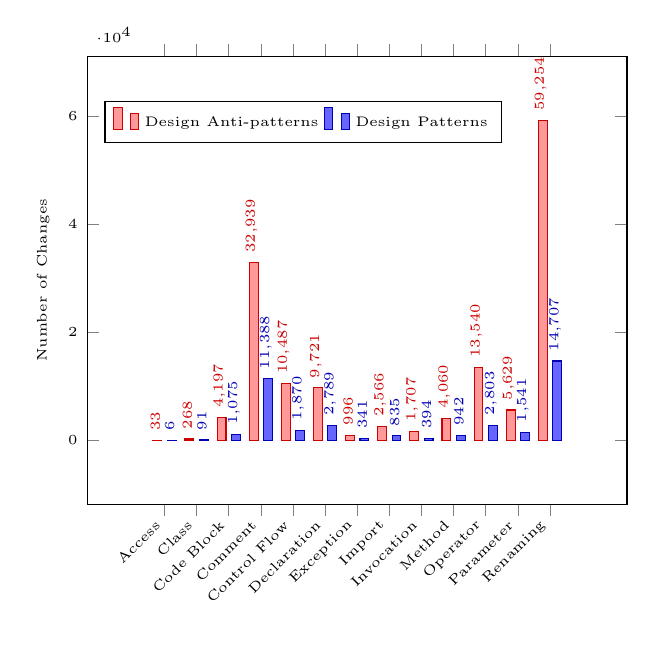
\begin{tikzpicture}
\pgfplotsset{every node/.append style={font=\tiny}}
\pgfplotsset{every tick label/.append style={font=\tiny}}
\begin{axis}[
    ybar,
    ymin=0,
    enlargelimits=0.2,
    legend style={at={(0.4,0.9)},anchor=north,legend columns=-1},
    bar width=1.12mm,
    ylabel={Number of Changes},
    symbolic x coords={Access, Class, Code Block, Comment, 
		Control Flow, Declaration, Exception, Import, Invocation, Method, Operator, Parameter, Renaming},
    xtick=data,
    x tick label style={rotate=45,anchor=east},
    nodes near coords,
    nodes near coords align={center},style={font=\tiny},
    every node near coord/.append style={rotate=90,anchor=south west,
    inner ysep=-1.75pt,}
    ]

\addplot [red!80!black,fill=red!40] coordinates {
(Access,33)
(Class,268) 
(Code Block,4197)
(Comment,32939)
(Control Flow,10487)
(Declaration,9721)
(Exception,996)
(Import,2566)
(Invocation,1707)
(Method,4060)
(Operator,13540)
(Parameter,5629)
(Renaming,59254)};
  
\addplot [blue!70!black,fill=blue!60] coordinates {
(Access,6) 
(Class,91)
(Code Block,1075) 
(Comment,11388)
(Control Flow,1870)
(Declaration,2789)
(Exception,341)
(Import,835)
(Invocation,394)
(Method,942)
(Operator,2803)
(Parameter,1541)
(Renaming,14707)};
\legend{Design Anti-patterns, Design Patterns}
\end{axis}
\end{tikzpicture}
}
\caption{Number of different types of changes in Eclipse classes with design anti-patterns and design patterns.}
\label{fig:FigureChangeEclipseNew}
\end{figure}

% Nuxeo
\begin{figure}
\centering
\scalebox{1.1}{
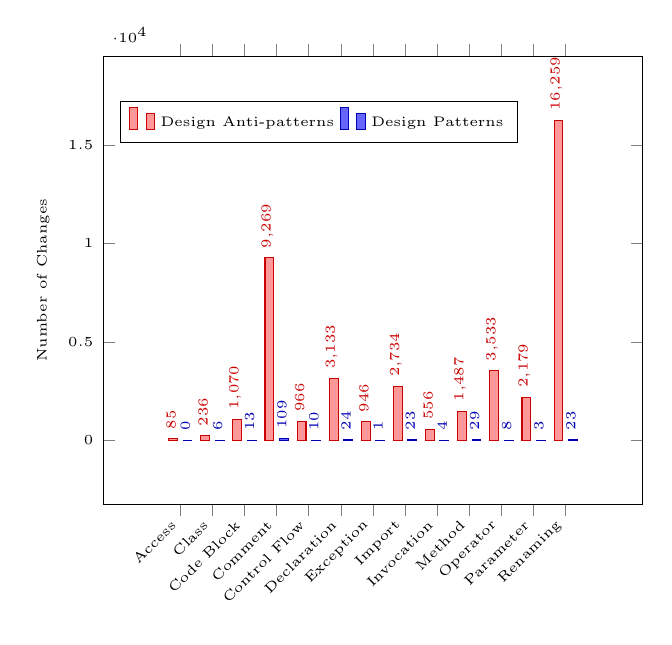
\begin{tikzpicture}
\pgfplotsset{every node/.append style={font=\tiny}}
\pgfplotsset{every tick label/.append style={font=\tiny}}
\begin{axis}[
    ybar,
    ymin=0,
    enlargelimits=0.2,
    legend style={at={(0.4,0.9)},anchor=north,legend columns=-1},
    bar width=1.12mm,
    ylabel={Number of Changes},
    symbolic x coords={Access, Class, Code Block, Comment, 
		Control Flow, Declaration, Exception, Import, Invocation, Method, Operator, Parameter, Renaming},
    xtick=data,
    x tick label style={rotate=45,anchor=east},
    nodes near coords,
    nodes near coords align={center},style={font=\tiny},
    every node near coord/.append style={rotate=90,anchor=south west,
    inner ysep=-1.75pt,}
    ]

\addplot [red!80!black,fill=red!40] coordinates {
(Access,85)
(Class,236) 
(Code Block,1070)
(Comment,9269)
(Control Flow,966)
(Declaration,3133)
(Exception,946)
(Import,2734)
(Invocation,556)
(Method,1487)
(Operator,3533)
(Parameter,2179)
(Renaming,16259)};
  
\addplot [blue!70!black,fill=blue!60] coordinates {
(Access,0) 
(Class,6)
(Code Block,13) 
(Comment,109)
(Control Flow,10)
(Declaration,24)
(Exception,1)
(Import,23)
(Invocation,4)
(Method,29)
(Operator,8)
(Parameter,3)
(Renaming,23)};
\legend{Design Anti-patterns, Design Patterns}
\end{axis}
\end{tikzpicture}
}
\caption{Number of different types of changes in Nuxeo classes with design anti-patterns and design patterns.}
\label{fig:FigureChangeNuxeoNew}
\end{figure}

% Ovirt
\begin{figure}
\centering
\scalebox{1.1}{
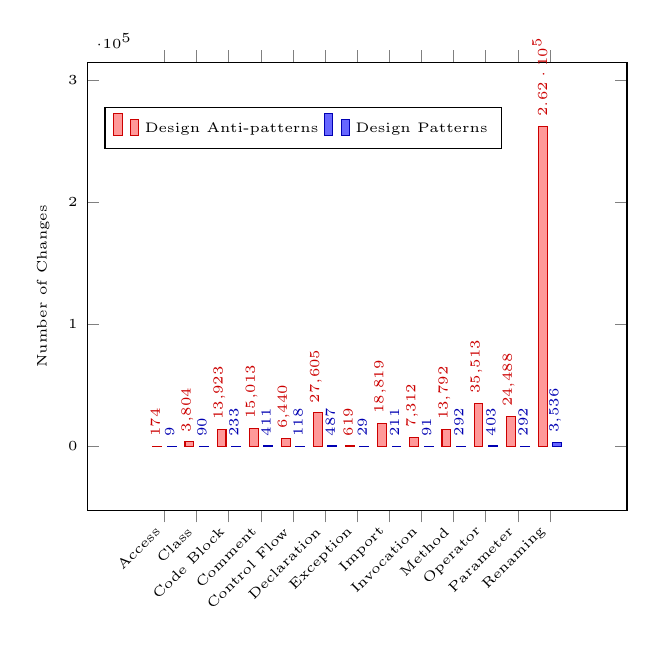
\begin{tikzpicture}
\pgfplotsset{every node/.append style={font=\tiny}}
\pgfplotsset{every tick label/.append style={font=\tiny}}
\begin{axis}[
    ybar,
    ymin=0,
    enlargelimits=0.2,
    legend style={at={(0.4,0.9)},anchor=north,legend columns=-1},
    bar width=1.12mm,
    ylabel={Number of Changes},
    symbolic x coords={Access, Class, Code Block, Comment, 
		Control Flow, Declaration, Exception, Import, Invocation, Method, Operator, Parameter, Renaming},
    xtick=data,
    x tick label style={rotate=45,anchor=east},
    nodes near coords,
    nodes near coords align={center},style={font=\tiny},
    every node near coord/.append style={rotate=90,anchor=south west,
    inner ysep=-1.75pt,}
    ]

\addplot [red!80!black,fill=red!40] coordinates {
(Access,174)
(Class,3804) 
(Code Block,13923)
(Comment,15013)
(Control Flow,6440)
(Declaration,27605)
(Exception,619)
(Import,18819)
(Invocation,7312)
(Method,13792)
(Operator,35513)
(Parameter,24488)
(Renaming,262491)};
  
\addplot [blue!70!black,fill=blue!60] coordinates {
(Access,9) 
(Class,90)
(Code Block,233) 
(Comment,411)
(Control Flow,118)
(Declaration,487)
(Exception,29)
(Import,211)
(Invocation,91)
(Method,292)
(Operator,403)
(Parameter,292)
(Renaming,3536)};
\legend{Design Anti-patterns, Design Patterns}
\end{axis}
\end{tikzpicture}
}
\caption{Number of different types of changes in oVirt classes with design anti-patterns and design patterns.}
\label{fig:FigureChangeoVirtNew}
\end{figure}

% Matsim
\begin{figure}
\centering
\scalebox{1.1}{
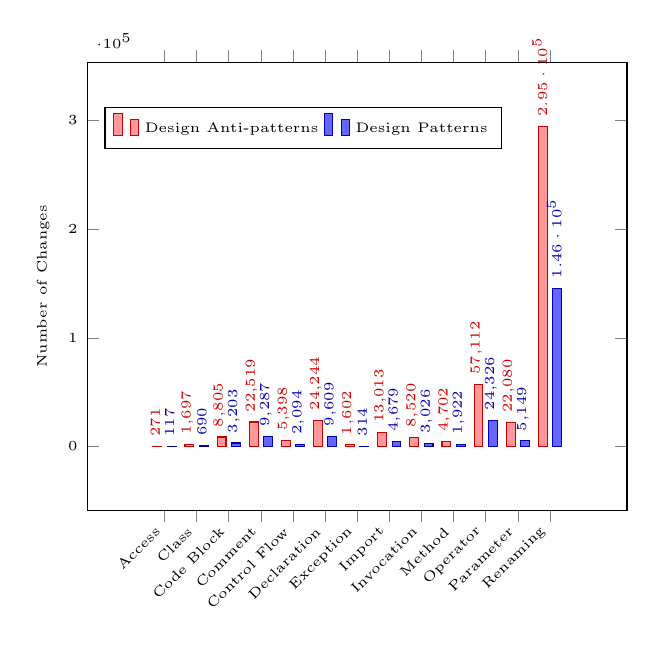
\begin{tikzpicture}
\pgfplotsset{every node/.append style={font=\tiny}}
\pgfplotsset{every tick label/.append style={font=\tiny}}
\begin{axis}[
    ybar,
    ymin=0,
    enlargelimits=0.2,
    legend style={at={(0.4,0.9)},anchor=north,legend columns=-1},
    bar width=1.12mm,
    ylabel={Number of Changes},
    symbolic x coords={Access, Class, Code Block, Comment, 
		Control Flow, Declaration, Exception, Import, Invocation, Method, Operator, Parameter, Renaming},
    xtick=data,
    x tick label style={rotate=45,anchor=east},
    nodes near coords,
    nodes near coords align={center},style={font=\tiny},
    every node near coord/.append style={rotate=90,anchor=south west,
    inner ysep=-1.75pt,}
    ]

\addplot [red!80!black,fill=red!40] coordinates {
(Access,271)
(Class,1697) 
(Code Block,8805)
(Comment,22519)
(Control Flow,5398)
(Declaration,24244)
(Exception,1602)
(Import,13013)
(Invocation,8520)
(Method,4702)
(Operator,57112)
(Parameter,22080)
(Renaming,294661)};
  
\addplot [blue!70!black,fill=blue!60] coordinates {
(Access,117) 
(Class,690)
(Code Block,3203) 
(Comment,9287)
(Control Flow,2094)
(Declaration,9609)
(Exception,314)
(Import,4679)
(Invocation,3026)
(Method,1922)
(Operator,24326)
(Parameter,5149)
(Renaming,145720)};
\legend{Design Anti-patterns, Design Patterns}
\end{axis}
\end{tikzpicture}
}
\caption{Number of different types of changes in Matsim classes with design anti-patterns and design patterns.}
\label{fig:FigureChangeMatsimNew}
\end{figure}

%ApacheIgnite
\begin{figure}
\centering
\scalebox{1.1}{
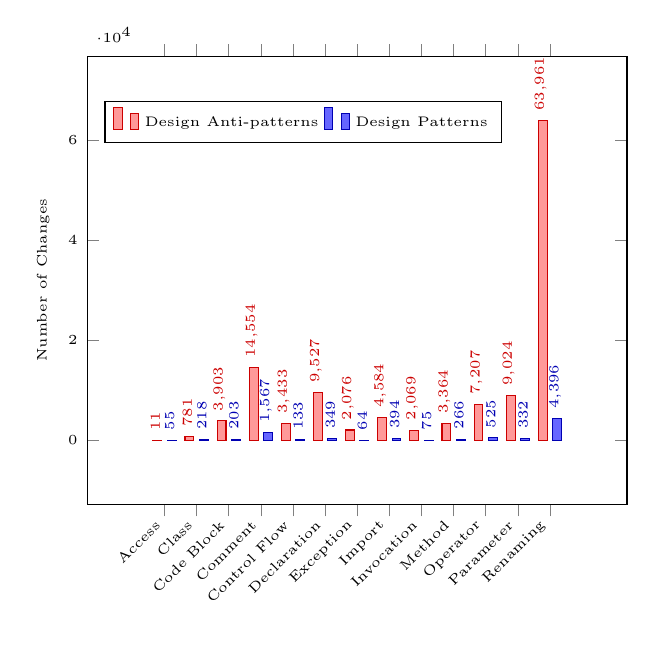
\begin{tikzpicture}
\pgfplotsset{every node/.append style={font=\tiny}}
\pgfplotsset{every tick label/.append style={font=\tiny}}
\begin{axis}[
    ybar,
    ymin=0,
    enlargelimits=0.2,
    legend style={at={(0.4,0.9)},anchor=north,legend columns=-1},
    bar width=1.12mm,
    ylabel={Number of Changes},
    symbolic x coords={Access, Class, Code Block, Comment, 
		Control Flow, Declaration, Exception, Import, Invocation, Method, Operator, Parameter, Renaming},
    xtick=data,
    x tick label style={rotate=45,anchor=east},
    nodes near coords,
    nodes near coords align={center},style={font=\tiny},
    every node near coord/.append style={rotate=90,anchor=south west,
    inner ysep=-1.75pt,}
    ]

\addplot [red!80!black,fill=red!40] coordinates {
(Access,11)
(Class,781) 
(Code Block,3903)
(Comment,14554)
(Control Flow,3433)
(Declaration,9527)
(Exception,2076)
(Import,4584)
(Invocation,2069)
(Method,3364)
(Operator,7207)
(Parameter,9024)
(Renaming,63961)};
  
\addplot [blue!70!black,fill=blue!60] coordinates {
(Access,55) 
(Class,218)
(Code Block,203) 
(Comment,1567)
(Control Flow,133)
(Declaration,349)
(Exception,64)
(Import,394)
(Invocation,75)
(Method,266)
(Operator,525)
(Parameter,332)
(Renaming,4396)};
\legend{Design Anti-patterns, Design Patterns}
\end{axis}
\end{tikzpicture}
}
\caption{Number of different types of changes in Apache Ignite classes with design anti-patterns and design patterns.}
\label{fig:FigureChangeApacheIgniteNew}
\end{figure}

%ApacheISolr
\begin{figure}
\centering
\scalebox{1.1}{
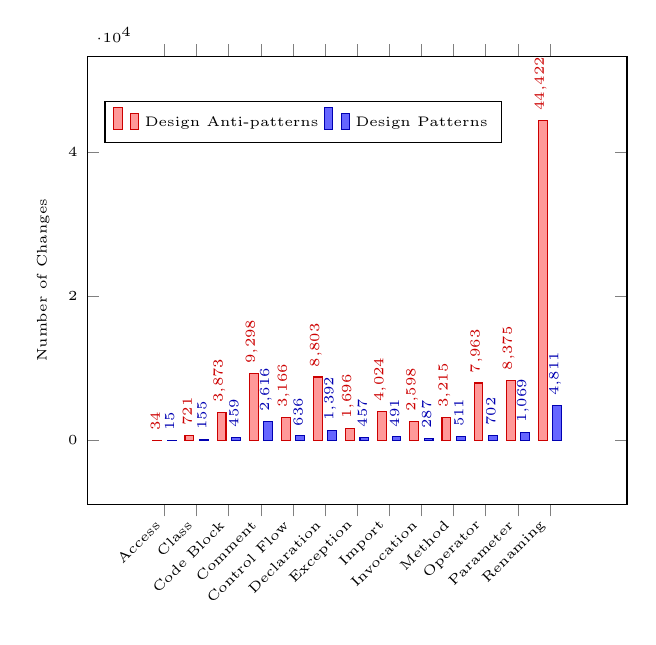
\begin{tikzpicture}
\pgfplotsset{every node/.append style={font=\tiny}}
\pgfplotsset{every tick label/.append style={font=\tiny}}
\begin{axis}[
    ybar,
    ymin=0,
    enlargelimits=0.2,
    legend style={at={(0.4,0.9)},anchor=north,legend columns=-1},
    bar width=1.12mm,
    ylabel={Number of Changes},
    symbolic x coords={Access, Class, Code Block, Comment, 
		Control Flow, Declaration, Exception, Import, Invocation, Method, Operator, Parameter, Renaming},
    xtick=data,
    x tick label style={rotate=45,anchor=east},
    nodes near coords,
    nodes near coords align={center},style={font=\tiny},
    every node near coord/.append style={rotate=90,anchor=south west,
    inner ysep=-1.75pt,}
    ]

\addplot [red!80!black,fill=red!40] coordinates {
(Access,34)
(Class,721) 
(Code Block,3873)
(Comment,9298)
(Control Flow,3166)
(Declaration,8803)
(Exception,1696)
(Import,4024)
(Invocation,2598)
(Method,3215)
(Operator,7963)
(Parameter,8375)
(Renaming,44422)};
  
\addplot [blue!70!black,fill=blue!60] coordinates {
(Access,15) 
(Class,155)
(Code Block,459) 
(Comment,2616)
(Control Flow,636)
(Declaration,1392)
(Exception,457)
(Import,491)
(Invocation,287)
(Method,511)
(Operator,702)
(Parameter,1069)
(Renaming,4811)};
\legend{Design Anti-patterns, Design Patterns}
\end{axis}
\end{tikzpicture}
}
\caption{Number of different types of changes in Apache Solr classes with design anti-patterns and design patterns.}
\label{fig:FigureChangeApacheSolrNew}
\end{figure}

% Mule
\begin{figure}
\centering
\scalebox{1.1}{
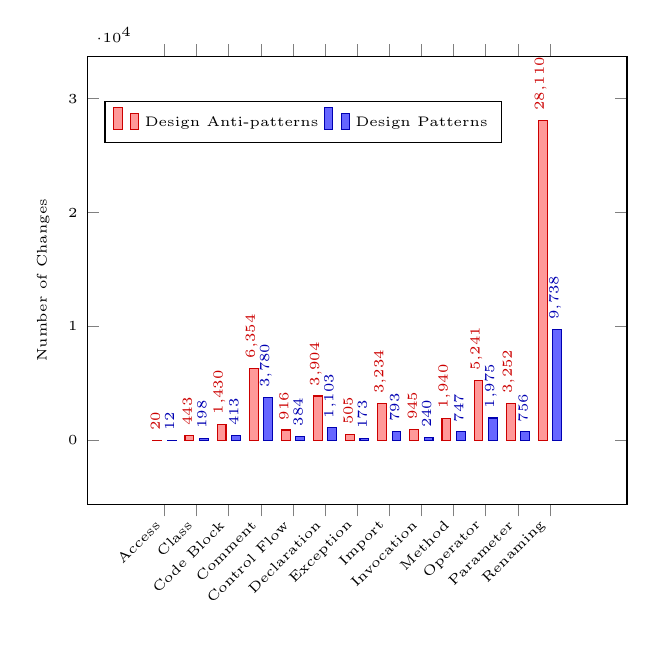
\begin{tikzpicture}
% \pgfplotsset{width = 10cm}
\pgfplotsset{every node/.append style={font=\tiny}}
\pgfplotsset{every tick label/.append style={font=\tiny}}
\begin{axis}[
    ybar,
    ymin=0,
    enlargelimits=0.2,
    legend style={at={(0.4,0.9)},anchor=north,legend columns=-1},
    bar width=1.12mm,
    ylabel={Number of Changes},
    symbolic x coords={Access, Class, Code Block, Comment, 
		Control Flow, Declaration, Exception, Import, Invocation, Method, Operator, Parameter, Renaming},
    xtick=data,
    x tick label style={rotate=45,anchor=east},
    nodes near coords,
    nodes near coords align={center},style={font=\tiny},
    every node near coord/.append style={rotate=90,anchor=south west,
    inner ysep=-1.75pt,}
    ]

\addplot [red!80!black,fill=red!40] coordinates {
(Access,20)
(Class,443) 
(Code Block,1430)
(Comment,6354)
(Control Flow,916)
(Declaration,3904)
(Exception,505)
(Import,3234)
(Invocation,945)
(Method,1940)
(Operator,5241)
(Parameter,3252)
(Renaming,28110)};
  
\addplot [blue!70!black,fill=blue!60] coordinates {
(Access,12) 
(Class,198)
(Code Block,413) 
(Comment,3780)
(Control Flow,384)
(Declaration,1103)
(Exception,173)
(Import,793)
(Invocation,240)
(Method,747)
(Operator,1975)
(Parameter,756)
(Renaming,9738)};
\legend{Design Anti-patterns, Design Patterns}
\end{axis}
\end{tikzpicture}
}
\caption{Number of different types of changes in Mule classes with design anti-patterns and design patterns.}
\label{fig:FigureChangeMuleNew}
\end{figure}

\paragraph{\textbf{Analysing change types of mutations}} During evolution, design patterns and design anti-patterns can mutate into other design patterns and design anti-patterns. We investigate which types of changes lead to such mutations. 
% The results of detected change types are contained in CSV files related to changed classes participating in design patterns and design anti-patterns for each system. Each CSV file includes the name of the two subsequent snapshots compared for change detection, the type of changes and the names of the classes changed. We compare two CSV files related to design patterns and design anti-patterns. By comparing the names of classes participating in occurrences of design patterns and design anti-patterns, we find the same class names which indicate that we have a mutation from design anti-patterns to design patterns and vice versa. 
Tables \ref{tab:dpapMutations} shows the number of each change types during the mutation for all the studied systems.

Results show that, in Apache Ignite, Renaming, Comment, and Declaration lead the most mutations from design anti-patterns (DAPs) to design patterns (DPs). It is almost the same for DPs-to-DAPs mutations but Parameter has more importance than Declaration. In Apache Solr and Eclipse for both DAPs-to-DPs and DPs-to-DAPs mutations, Renaming, Declaration, and Comment are the most representative change types. In Matsim, Renaming, Operator, and Declaration have the most impact on DAPs-to-DPs mutations while Renaming, Comment, and Operator lead to more DPs-to-DAPs mutations. In Mule, for both DAPs-to-DPs and DPs-to-DAPs mutations, Renaming, Comment, and Operator are the most representative change types. In Nuxeo, there are few mutations, in which Comment, Renaming, and Declaration yield DAPs-to-DPs mutations while Comment, Code Block, and Control Flow yield more DPs-to-DAPs mutations. Finally, in oVirt, Renaming, Declaration, and Comment are change types that lead to DAPs-to-DPs mutations while Renaming, Operator, and Declaration bring DPs-to-DAPs mutations.

Renaming is the most frequent change type. There are different types of renaming, described in \cite{arnaoudova2014repent}. In some types, an entity, \eg{} a package, a class, etc., is renamed. In other types, one or more terms are changed (simple and complex renaming). Sometimes, when one or more terms change, the meaning of the identifier also changes (semantic renaming). The grammar of an identifier may also change during evolution (grammar renaming). When developers use some tools to apply a renaming operation, the tool may not rename all variables consistently in all related files. Besides, certain source-code changes must be made together to preserve consistency. Changes in comments and declarations led to more mutations not as root causes of these mutations but because developers changed comments and declarations while evolving their systems for other reasons, \ie{} fixing faults. Future work include a manual, qualitative analysis of the mutations to identify their root causes.

\begin{tcolorbox}
\vspace{-0.1cm}
\textbf{Summary:} \emph{Some change types affect the mutations between design patterns and--or design anti-patterns more than others. We observe that the change types leading to mutations in all the studied systems are Renaming, Comment, Declaration, and Operator.}
\vspace{-0.1cm}
\end{tcolorbox}



\subsection{\textbf{RQ3:} \textit{\RQThree}}

\paragraph{\textbf{Motivation}} The results from RQ1 and RQ2 show that design patterns and design anti-patterns mutate during software evolution. However, they do not say anything about the impact of these mutations in software quality. Therefore, we investigate these mutations and their fault-proneness. Using this information, developers could understand the reasons of faults and take actions to reduce the risk of introducing faults.

\paragraph{\textbf{Analysing design patterns and design anti-patterns fault-proneness}} For each system, we mine its commit log and extract fault and commit IDs related to the faults and the dates when the faults were introduced. We look for faults introduced from one snapshot to the next. We use the dates to distinguish between faults appearing in one snapshot and those appearing between two extracted snapshots.

Table \ref{tab:DAP-DPfault} shows the numbers of faulty and clean of classes involved in patterns. One class can be involved in several faults in the studied snapshots so we show in Table \ref{tab:fault} the numbers of unique faulty and clean classes involved in patterns. Finally, in Table \ref{tab:faultpercentages}, we compare the percentages of faulty and clean classes involved in design patterns and design anti-patterns. Moreover, we show in Table \ref{tab:faultpercentages} the relative percentages of faults per class participating, or not, in design (anti-)patterns. 

With these tables, we summarise our whole dataset with: the numbers of (unique) faulty and non-faulty (clean) classes participating or not in design (anti-)patterns and their relative percentages. We thus can compare the prevalence of faults in different classes and confirm that classes participating in design anti-patterns have more faults than classes involved in design patterns. Thus, we have evidence supporting that classes that participate in design anti-patterns are more fault-prone than classes involved in design patterns.

For example, in Eclipse, 13.7\% of design pattern classes are fault-prone while 37.3\% of design anti-pattern classes are fault-prone. Table \ref{tab:faultpercentages} is showing similar trends in all the analysed systems.

\begin{table*} [ht]
\centering
\caption{Design anti-pattern and design-pattern mutations between faulty and clean classes}
\scalebox{0.8}{
\renewcommand{\arraystretch}{1.1}
\begin{tabular}{|l|r|r|r|}
\hline
\multirow{2}{*}{\textbf{\textbf{Systems}}} & \multicolumn{2}{c|}{\textbf{\# of Faulty classes}} & \multirow{2}{*}{\textbf{\# of Clean classes having DAPs, DPs}} \\
\cline{2-3}
 & Design Anti-patterns & Design Patterns & \\
 \hline \hline
 Apache Ignite & 10,984 & 1,051 & 81,093\\ 
 \hline
 Apache Solr & 11,156 & 219 & 109,225 \\
 \hline
 Eclipse & 15,240 & 5,182 & 19,928 \\
\hline
 Matsim & 4,053 & 1,888 & 896,510 \\
\hline
 Mule & 17,794 & 5,924 & 197,574 \\
\hline
 Nuxeo & 18,724 & 396 & 146,180 \\
\hline
 oVirt & 12,605 & 110 & 217,565 \\
\hline
\end{tabular}
}
\label{tab:DAP-DPfault}
\end{table*} 

\begin{table*} [ht]
\centering
\caption{Faulty and clean classes}
\scalebox{0.7}{
\renewcommand{\arraystretch}{1.1}
\begin{tabular}{|l|rr|rr|rr|rr|rr|}
\hline
\multirow{2}{*}{\textbf{Systems}} & \multicolumn{4}{c|}{\textbf{\# of Faulty Classes}} & \multicolumn{2}{c|}{\textbf{\# of Faulty Classes}} & \multicolumn{4}{c|}{\textbf{\# of Clean Classes}} \\
\cline{2-11}
& \multicolumn{2}{c|}{DAPs} & \multicolumn{2}{c|}{DPs} & \multicolumn{2}{c|}{\textbf{without Patterns}} & \multicolumn{2}{c|}{DAPs} &
\multicolumn{2}{c|}{DPs} \\
\hline \hline
Apache Ignite & 10,984 & (685) & 1,051 & (84) & 3,984 & (3,984) & 71,784 & (3,474) & 9,309 & (395)\\
\hline
Apache Solr & 11,156 & (638) & 219 & (22) & 6,351 & (6,351) & 101,044 & (3,447) & 8,181 & (392)\\
\hline
Eclipse & 15,240 & (591) & 5,182 & (217) & 12,285 & (12,285) & 13,610 & (562) & 6,318 & (213)\\
\hline
Matsim & 4,053 & (469) & 1,888 & (115) & 291 & (291) & 326,460 & (14,425) & 570,050 & (9,913)\\
\hline
Mule & 17,794 & (2,955) & 5,924 & (196) & 4,370 & (4,370) & 126,980 & (7,341) & 70,594 & (1,593)\\
\hline
Nuxeo & 18,724 & (1,487) & 396 & (68) & 7,414 & (7,414) & 143,276 & (3,659) & 2,904 & (170)\\
\hline
oVirt & 12,605 & (377) & 110 & (8) & 523 & (523) & 214,027 & (7,653) & 3,538 & (214)\\
\hline
\end{tabular}
}
\label{tab:fault}
\end{table*} 

\begin{table*} [ht]
\centering
\caption{Faulty and clean classes in percentages}
\scalebox{0.7}{
\renewcommand{\arraystretch}{1.1}
\begin{tabular}{|l|r|r|r|r|}
\hline
\multirow{2}{*}{\textbf{Systems}} & \multicolumn{2}{c|}{\textbf{Design anti-patterns}} & \multicolumn{2}{c|}{\textbf{Design patterns}} \\
\cline{2-5}
& Faulty Classes (\%) & Clean Classes (\%) &
Faulty Classes (\%) & Clean Classes (\%) \\
\hline \hline
Apache Ignite & 14.7\% & 74.9\% & 1.8\% & 8.5\% \\
\hline
Apache Solr & 14.1\% & 76.6\% & 0.48\% & 8.7\% \\
\hline
Eclipse & 37.3\% & 35.5\% & 13.7\% & 13.4\% \\
\hline
Matsim & 1.9\% & 57.9\% & 0.46\% & 39.7\% \\
\hline
Mule & 24.4\% & 60.7\% & 1.6\% & 13.2\% \\
\hline
Nuxeo & 27.6\% & 67.9\% & 1.3\% & 3.2\%\\
\hline
oVirt & 4.6\% & 92.7\% & 0.09\% & 2.6\%\\
\hline
\end{tabular}
}
\label{tab:faultpercentages}
\end{table*} 



\paragraph{\textbf{Analyzing mutations fault-proneness}} A mutation between design patterns and design anti-patterns can lead to faults. We use clean and faulty classes and their participation (or not) into design patterns and design anti-patterns to identify the mutations experienced by these faulty classes.

Table \ref{tab:TransFault} presents the most representative mutations that led to faults in each studied system. We observe that mutations from design anti-patterns to other design anti-patterns are more faulty. LongParameterList to LongMethod or LongMethod to LazyClass are such mutations in Apache Ignite. 

In Eclipse, Matsim, and Mule, there are mutations from design patterns to design patterns that also led to more faults. FactoryMethod to Decorator in Eclipse, Builder to FactoryMethod in Matsim and Mule are such mutations. 

There are also mutations from design anti-patterns to design patterns that led to faults as well, like AntiSingleton to FactoryMethod in Matsim or FactoryMethod to LongMethod in Eclipse. 

% Design anti-patterns are introduced by ``bad” implementations or design choices and such choices are implementing or designing a (or part of a) class. This could make the classes very large and complex leading to comprehension overheads to the developers. On the other hand, design patterns are good solutions to solve the design and implementation problems in the classes. Thus, the classes containing design anti-patterns are likely to be more fault-prone than classes containing design patterns; which is supported by our findings.

\begin{table*} [ht]
\centering
\caption{Most representative mutations between design patterns and design anti-patterns according to their mutation probabilities and fault-proneness}

\scalebox{0.8}{
\renewcommand {\arraystretch} {1.1}
\begin{tabular}{|l|l|l|l|r|}
\hline
\textbf{System} & \textbf{Mutation Type} & \textbf{From}  & \textbf{To} & \textbf{Probability} \\ \hline
\hline
\multirow{2}{*}{Apache Ignite} & 
 DAP$\,\to\,$DAP & LongParameterList & LongMethod & 0.571\\
\cline{2-5}
& DAP$\,\to\,$DAP & LongMethod & LazyClass & 0.285\\
\cline{2-5}
\hline
\multirow{3}{*}{Apache Solr} &  DAP$\,\to\,$DAP & RefusedParentBequest & MessageChain & 0.427\\
\cline{2-5}
& DAP$\,\to\,$DAP & LongMethod & LazyClass & 0.156 \\
\cline{2-5}
& DAP$\,\to\,$DAP & ComplexClass & ClassDataShouldBePrivate & 0.156\\
\cline{2-5}
\hline 
\multirow{3}{*}{Eclipe IDE} &  
 DP$\,\to\,$DP & FactoryMethod & Decorator & 0.492\\
 \cline{2-5} 
  & DAP$\,\to\,$DAP & LongMethod & LazyClass & 0.385\\
\cline{2-5}
 & DP$\,\to\,$DAP & FactoryMethod & LongMethod & 0.056\\
\cline{2-5}
\hline 
\multirow{3}{*}{Matsim} & 
DP$\,\to\,$DP & Builder & FactoryMethod & 0.677\\
\cline{2-5}
& DAP$\,\to\,$DAP & SpagettiCode & RefusedParentBequest & 0.152\\
\cline{2-5}
 & DAP$\,\to\,$DP & AntiSingleton & FactoryMethod & 0.114\\
\cline{2-5}
\hline 
\multirow{3}{*}{Mule} & 
DP$\,\to\,$DP & Builder & FactoryMethod & 0.479 \\
\cline{2-5}
& DAP$\,\to\,$DP & ComplexClass & FactoryMethod & 0.264\\
\cline{2-5}
& DAP$\,\to\,$DAP & ComplexClass & ClassDataShouldBePrivate & 0.223\\ 
\cline{2-5}
\hline  
\multirow{2}{*}{Nuxeo} & DAP$\,\to\,$DAP & LazyClass & LargeClass & 0.285\\
\cline{2-5}
 & DP$\,\to\,$DP & Singleton & FactoryMethod & 0.495\\
\hline 
\multirow{2}{*}{oVirt} & DAP$\,\to\,$DAP & Blob & AntiSingleton & 0.722\\ 
\cline{2-5}
 & DP$\,\to\,$DP & Singleton & Prototype& 0.166\\ 
\hline 
\end{tabular}
}
\label{tab:TransFault}
\end{table*} 

\begin{tcolorbox}
\vspace{-0.1cm}
\textbf{Summary:} \emph{We observed that in some systems, as expected and shown in previous work, design anti-patterns are more fault-prone than design patterns. We also showed that some mutations are more fault-prone than others, in particular mutations from design anti-patterns to design patterns or to other design anti-patterns.}
\vspace{-0.1cm}
\end{tcolorbox}



\subsection{\textbf{RQ4:} \textit{\RQFour}}

\paragraph{\textbf{Motivation}} Different types of changes have different impacts on the software systems due to their differences in functionality and the ripple effects of changes. Some types of changes likely introduce more faults than others. Thus, understanding which types of changes increase the fault-proneness of the mutations could help developers to foresee and prevent faults by preventing/planning such changes during software evolution.

\paragraph{\textbf{Analysing change types leading to faults}} We use the same data as in RQ2 and RQ3. For each system, we identify the number of faulty classes that have changed through mutations between design anti-patterns and--or design patterns. Table \ref{tab:ChangeAn2De} shows the number of change types that led to faults. We report that, in all studied systems, Renaming, Comment, and Operator are the change types that lead to more faults.

\begin{table*}[ht]
\centering
\caption{Numbers of change types in the studied systems leading to faults} \label{tab:noFaultyChanges}
\scalebox{0.71}{
\renewcommand{\arraystretch}{1.1}
\begin{tabular}{|p{2.1cm}|r|r|r|r|r|r|r|}\hline
\textbf{Systems $\rightarrow$ }& \textbf{Apache Ignite} & \textbf{Apache Solr} & \textbf{Eclipse~~~} & \textbf{Matsim~~~} & \textbf{Mule~~~} & \textbf{Nuxeo~~~} & \textbf{oVirt~~~}\\\hline
\textbf{\textbf{Change Types}} &\# changes  &\# changes&\# changes &\# changes & \# changes &\# changes &\# changes\\
\hline \hline
  Access &18  &18  & 37 & 22 & 11 & 62 & 25\\ \hline
  Class &689  &431  &306  &306  & 422 &208  &763 \\ \hline
  Code block & 2,972 & 2,102 & 4,919 & 1,284 &1,306  & 854 & 3,833\\ \hline
  Comment & 12,169 & 5,498 & 38,150 & 2,813 & 6,270 &6,161  &4,653 \\ \hline
  Control flow &2,903  & 1,935 & 11,678 & 660 &  1067& 819 &2,406 \\ \hline
  Declaration &5,912  &  5,386& 11651 &  3,129& 3,191 & 2,628 &7,484 \\ \hline
  Exception &1,696  & 1221 & 1255 & 140 &  526& 786&  210\\ \hline
  Import & 2,831 &2,400  &2,958  & 1,425 &2,443  & 2,064 & 4,268 \\ \hline
  Invocation &1,550  &1,196  & 1,986 & 1,061 & 840 & 476 &1,882 \\ \hline
  Method & 2,509 & 1,851 & 4,093 &637  & 1,697 & 1,229 & 3,619\\ \hline
  Operator &5,120  & 4,364 & 16,094 & 6,215 & 4,228 & 2,675 & 8,134\\ \hline
  Parameter & 6,418 & 3,504 & 5,108 & 2,655 & 2,607 & 1,815 & 5,337 \\ \hline
  Renaming & 47,811 & 24,640 & 67,040 & 32,445 & 22,968 &  12,736& 65,245 \\ \hline
  \textbf{Total changed classes} &  5,505& 4,163 & 11,934 & 3,073 & 4,324 & 3,514 &7,150 \\ \hline
\end{tabular}
}
\label{tab:ChangeAn2De}
\end{table*} 

\paragraph{\textbf{Analyzing fault-proneness of classes with design patterns and design anti-patterns}} Table \ref{tab:Changefault} presents the numbers of faulty changed classes and Figures \ref{fig:DPFaultyChangedClasses} and \ref{fig:APFaultyChangedClasses} show the percentages of faulty changed classes participating in design patterns and design anti-patterns for all the systems. Figure \ref{fig:AP_DPFaultyChangedClasses} compares the numbers of faulty and clean classes changed in all the snapshots of the studied systems. Each first bar presents the number of faulty and clean changed classes participating in design anti-patterns and the second one is faulty and clean classes having design patterns. We observe that change types have impacts on the fault-proneness of changed classes. Changed classes participating in design patterns are less faulty than those participating only in design anti-patterns. 

Figures \ref{fig:DPFaultyChangedClasses} and \ref{fig:APFaultyChangedClasses} show that some of the faulty classes are those which had changed in the past. For example, in Eclipse, the percentages of faulty classes participating in design patterns is 81\% while for those participating in design anti-patterns it is 86\%. The differences between these two categories are more visible in Apache Solr, where 51\% of changed classes are participating in design anti-patterns, and only 11\% of them have design patterns. In Rhino, changes impact fault-proneness significantly, because, on average, more than 85\% of changed classes are faulty. Thus, the trend is that changed classes with design anti-patterns tend to be more fault-prone than changed classes with design patterns.

\begin{table*} [ht]
\centering
\caption{Numbers of faulty and clean changed classes}
\scalebox{0.9}{
\renewcommand{\arraystretch}{1.1}
\begin{tabular}{|l|l|r|r|}
\hline
\textbf{Systems} & \textbf{Patterns}  & \textbf{\# Faulty classes} & \textbf{\# Clean classes}\\
\hline \hline
\multirow{2}{*}{Apache Ignite} & Design Anti-patterns & 5,112 & 4,178\\ 
 \cline{2-4}
 & Design Patterns & 393 & 464\\
\hline
\multirow{2}{*}{Apache Solr} & Design Anti-patterns & 4,035 & 3,921\\
\cline{2-4}
 & Design patterns & 128 & 1,064\\
\hline
\multirow{2}{*}{Eclipse} & Design Anti-patterns & 9,406 & 1,551\\
\cline{2-4}
 & Design patterns & 2,554 & 601\\
\hline
\multirow{2}{*}{Matsim} & Design Anti-patterns & 2,549 & 30,042\\
\cline{2-4}
 & Design patterns & 524 & 13,244\\
\hline
\multirow{2}{*}{Mule} & Design Anti-patterns & 3,374 & 2,311\\
\cline{2-4}
 & Design patterns & 950 & 1,225\\
\hline
\multirow{2}{*}{Nuxeo} & Design Anti-patterns & 3,469 & 1,935\\
\cline{2-4}
 & Design patterns & 45 & 36\\
\hline
\multirow{2}{*}{oVirt} & Design Anti-patterns & 7,075 & 27,705\\
\cline{2-4}
 & Design patterns & 75 & 482\\
\hline
\end{tabular}
}
\label{tab:Changefault}
\end{table*} 


\begin{figure}[ht]
\centering
\scalebox{0.8}{
  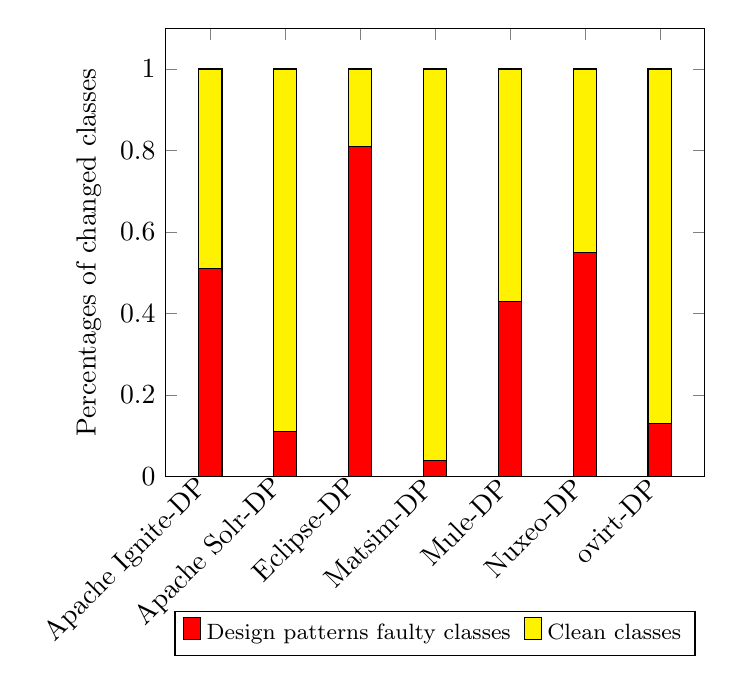
\begin{tikzpicture}
  \begin{axis}[
      every node near coord/.style={
     },
     legend style={
       font=\footnotesize,
       cells={anchor=east},
       legend columns=5,
       at={(0.50,-0.30)},
       anchor=north,
       /tikz/every even column/.append style={column sep=0.1cm}
     },
    title={},
    ybar stacked, ymin=0,
    bar width=3mm,
    ylabel={Percentages of changed classes},
    symbolic x coords=     {Apache Ignite-DP, Apache Solr-DP, Eclipse-DP, Matsim-DP, Mule-DP, Nuxeo-DP, ovirt-DP},
    xtick=data,
    x tick label style={rotate=45,anchor=east},
]
  %F
  \addplot [fill=red] coordinates {
%  ({Apache Ignite-AP},0.55)
  ({Apache Ignite-DP},0.51)
%  ({Apache Solr-AP},0.51)
  ({Apache Solr-DP},0.11)
%  ({Eclipse-AP},0.86)
  ({Eclipse-DP},0.81)
%  ({Matsim-AP},0.08)
  ({Matsim-DP},0.04)
%  ({Mule-AP},0.59)
  ({Mule-DP},0.43)
%  ({Nuxeo-AP},0.64)
  ({Nuxeo-DP},0.55)
%  ({Ovirt-AP},0.20)
  ({ovirt-DP},0.13)
};
    \addplot [fill=yellow] coordinates {
%  ({Apache Ignite-AP},0.45)
  ({Apache Ignite-DP},0.49)
%  ({Apache Solr-AP},0.49)
  ({Apache Solr-DP},0.89)
%  ({Eclipse-AP},0.14)
  ({Eclipse-DP},0.19)
%  ({Matsim-AP},0.92)
  ({Matsim-DP},0.96)
%  ({Mule-AP},0.41)
  ({Mule-DP},0.57)
%  ({Nuxeo-AP},0.36)
  ({Nuxeo-DP},0.45)
%  ({Ovirt-AP},0.80)
  ({ovirt-DP},0.87)
};
  \legend {Design patterns faulty classes, Clean classes} 
  \end{axis}
  \end{tikzpicture}
  }
 \caption{Faulty changed classes percentages with design pattern in the studied systems} 
\label{fig:DPFaultyChangedClasses}
\end{figure}

\begin{figure}[ht]
\centering
\scalebox{0.8}{
  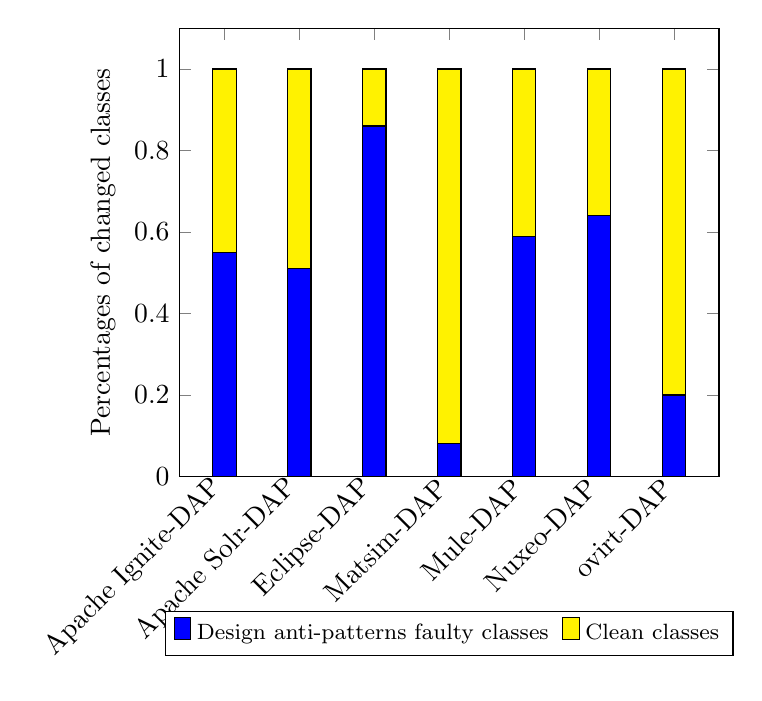
\begin{tikzpicture}
  \begin{axis}[
      every node near coord/.style={
     },
     legend style={
       font=\footnotesize,
       cells={anchor=east},
       legend columns=5,
       at={(0.50,-0.30)},
       anchor=north,
       /tikz/every even column/.append style={column sep=0.1cm}
     },
    title={},
    ybar stacked, ymin=0,
    bar width=3mm,
    ylabel={Percentages of changed classes},
    symbolic x coords=     {Apache Ignite-DAP, Apache Solr-DAP, Eclipse-DAP, Matsim-DAP, Mule-DAP, Nuxeo-DAP, ovirt-DAP},
    xtick=data,
    x tick label style={rotate=45,anchor=east},
]
  %F
  \addplot [fill=blue] coordinates {
  ({Apache Ignite-DAP},0.55)
%  ({Apache Ignite-DP},0.51)
  ({Apache Solr-DAP},0.51)
%  ({Apache Solr-DP},0.11)
  ({Eclipse-DAP},0.86)
%  ({Eclipse-DP},0.81)
  ({Matsim-DAP},0.08)
%  ({Matsim-DP},0.04)
  ({Mule-DAP},0.59)
%  ({Mule-DP},0.43)
  ({Nuxeo-DAP},0.64)
%  ({Nuxeo-DP},0.55)
  ({ovirt-DAP},0.20)
%  ({Ovirt-DP},0.13)
};

  \addplot [fill=yellow] coordinates {
  ({Apache Ignite-DAP},0.45)
%  ({Apache Ignite-DP},0.49)
  ({Apache Solr-DAP},0.49)
%  ({Apache Solr-DP},0.89)
  ({Eclipse-DAP},0.14)
%  ({Eclipse-DP},0.19)
  ({Matsim-DAP},0.92)
%  ({Matsim-DP},0.96)
  ({Mule-DAP},0.41)
%  ({Mule-DP},0.57)
  ({Nuxeo-DAP},0.36)
%  ({Nuxeo-DP},0.45)
  ({ovirt-DAP},0.80)
%  ({Ovirt-DP},0.87)
};
  \legend {Design anti-patterns faulty classes, Clean classes} 
  \end{axis}
  \end{tikzpicture}
  }
 \caption{Faulty changed classes with design anti-patterns percentages in the studied systems} 
\label{fig:APFaultyChangedClasses}
\end{figure}

\begin{figure}
\centering
\scalebox{1.1}{
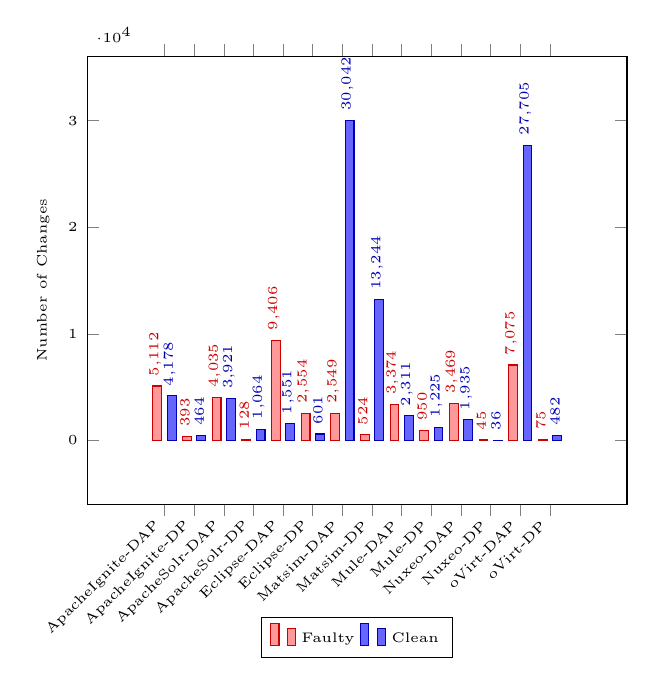
\begin{tikzpicture}
\pgfplotsset{every node/.append style={font=\tiny}}
\pgfplotsset{every tick label/.append style={font=\tiny}}
\begin{axis}[
    ybar,
    ymin=0,
    enlargelimits=0.2,
    legend style={at={(0.5,-0.25)},anchor=north,legend columns=-1},
    bar width=1.12mm,
    ylabel={Number of Changes},
    symbolic x coords={ApacheIgnite-DAP, ApacheIgnite-DP, ApacheSolr-DAP, ApacheSolr-DP, Eclipse-DAP, Eclipse-DP, Matsim-DAP, Matsim-DP, Mule-DAP, Mule-DP, Nuxeo-DAP, Nuxeo-DP, oVirt-DAP, oVirt-DP},
    xtick=data,
    x tick label style={rotate=45,anchor=east},
    nodes near coords,
    nodes near coords align={center},style={font=\tiny},
    every node near coord/.append style={rotate=90,anchor=south west,
    inner ysep=-1.75pt,}
    ]

\addplot [red!80!black,fill=red!40] coordinates {
(ApacheIgnite-DAP,5112) (ApacheIgnite-DP,393) (ApacheSolr-DAP,4035) (ApacheSolr-DP,128) (Eclipse-DAP,9406) (Eclipse-DP,2554) (Matsim-DAP,2549) (Matsim-DP,524) (Mule-DAP,3374) (Mule-DP,950) (Nuxeo-DAP,3469) (Nuxeo-DP,45) (oVirt-DAP,7075) (oVirt-DP,75)};
  
\addplot [blue!70!black,fill=blue!60] coordinates {
(ApacheIgnite-DAP,4178) (ApacheIgnite-DP,464) (ApacheSolr-DAP,3921) (ApacheSolr-DP,1064) (Eclipse-DAP,1551) (Eclipse-DP,601) (Matsim-DAP,30042) (Matsim-DP,13244) (Mule-DAP, 2311) (Mule-DP,1225) (Nuxeo-DAP,1935) (Nuxeo-DP,36) (oVirt-DAP,27705) (oVirt-DP,482)};
\legend{Faulty, Clean}
\end{axis}
\end{tikzpicture}
}
\caption{Faulty changed classes with design anti-patterns and design patterns in the studied systems} 
\label{fig:AP_DPFaultyChangedClasses}
\end{figure}

\begin{tcolorbox}
\vspace{-0.1cm}
\textbf{Summary:} \emph{Some change types applied to design patterns and design anti-patterns make software systems more fault-prone compared to others. We observed that, in all the studied systems, Renaming, Comment, and Operator are the change types from design patterns to design anti-patterns that most lead to faults.}
\vspace{-0.1cm}
\end{tcolorbox}